\documentclass[journal]{./IEEE/IEEEtran}
\usepackage{cite,graphicx}

\newcommand{\SPTITLE}{PARA!: A Multimodal Trip Planning Travel Companion and Public Transit Information System}
\newcommand{\ADVISEE}{Jonas R. Atienza}
\newcommand{\ADVISER}{Concepcion L. Khan}

\newcommand{\BSCS}{Bachelor of Science in Computer Science}
\newcommand{\ICS}{Institute of Computer Science}
\newcommand{\UPLB}{University of the Philippines Los Ba\~{n}os}
\newcommand{\REMARK}{\thanks{Presented to the Faculty of the \ICS, \UPLB\
                             in partial fulfillment of the requirements
                             for the Degree of \BSCS}}
        
\markboth{CMSC 190 Special Problem, \ICS}{}
\title{\SPTITLE}
\author{\ADVISEE~and~\ADVISER%
\REMARK
}
\pubid{\copyright~2024~ICS \UPLB}

%%%%%%%%%%%%%%%%%%%%%%%%%%%%%%%%%%%%%%%%%%%%%%%%%%%%%%%%%%%%%%%%%%%%%%%%%%

\begin{document}

% TITLE
\maketitle

% ABSTRACT
\begin{abstract}
Public transportation is a leading mode of transportation in the Philippines, but the public transportation system has often been criticized for lagging behind the standards of developed countries.
There is a lack of travel applications specifically tailored for public transportation assistance, and the current choices are limited and have limitations.
The goal of this paper is to develop the basis of a `commuter first' multimodal trip planning travel companion for mobile devices that commuters can use on demand and anywhere.
This is especially important for first-time commuters to an area.
Similarly, community-driven input is also important in molding a standardized transit feed dataset.
To leverage this need, the application will give users power to request the creation and modification of routes.
This project has the potential to improve the Quality of Life (QoL) of many commuters, especially those who are first time commuters to a certain place.
It can also help commuters be aware of traffic congestions and make the proper decisions in exploring other possible and more efficient routes. 
\end{abstract}

% INDEX TERMS
\begin{keywords}
public transport, transportation assistance, osm, osrs, leaflet, mobile development, flutter, google maps, commuting, cross-platform, android, ios
\end{keywords}

% INTRODUCTION
\section{Introduction}
Transportation plays an important part in the life of the modern man. In the Philippines, public transportation is a leading mode of transportation---having a predominant number of registered Public Utility Vehicles (PUVs) as opposed to privately-owned Motor Vehicles (MVs).
%[INSERT UPDATED DATA/CITATION HERE;\ Current data from 2020, request from eFOI still pending].
Mass public transportation is also cheaper, relatively convenient, and can sometimes be faster than private modes of transportation~\cite{Narboneta16}.

However, the public transportation system in the Philippines has often been criticized for lagging behind the standards of developed countries, leading to a negative perception of its convenience and overall experience. Despite these challenges, the benefits of an efficient and well-organized public transport system cannot be ignored---both for the benefit of the people and for the benefit of a greener world~\cite{Lagua19}.

Currently, Metro Manila is the only city in the Philippines which has a formal public transport---namely, the Light Rail Transit (LRT) and the Metro Rail Transit (MRT). Other cities and municipalities are only mostly catered by buses and other privately-owned---and operated---informal modes of transportation such as \textit{jeepney}, van, \textit{`tricycle'} (auto rickshaws), \textit{`pedicab'} (cycle rickshaws), and \textit{`habal-habal'} (motorcycles-for-hire)~\cite{Mayo20}.
These---on some cities---are nowadays accompanied by the Modern Public Utility Vehicles (MPUVs) and Modern Public Utility Jeepneys (MPUJs) brought by the Public Utility Vehicle Modernization Program (PUVMP) of the Department of Transportation (DOTr) as issued in Department Order (D.O.) No. 2017--011. %[ citation format for department order (?) ]

% NOTE: Check bib file for department order citation correctness.

\subsection{Background of the study}
Conventional Public Transport (CPT) is a mode of transport that is the backbone of transportation in the Philippines. It is recognized by law and by the public as the `standard' in the transport system. CPT covers the aforementioned \textit{jeepney}, van, \textit{`tricycle'}, \textit{`pedicab'}, \textit{`habal-habal'}, and train systems~\cite{RamizoJr19}.
`Conventional taxi'---such as the taxi systems in Metro Manila, Baguio City, etc.\---while under CPT, could be said to be distinct to the definition of CPT outlined in this paper, along with similar `ride hailing' services---such as GrabTaxi and Angkas, among others---since taxi services operate in a `pick up and drop off system' instead of adhering to a standard operating route.

The routes of each CPT mode have loops that are unique---albeit with some trips overlapping the routes of other trips. Each Trip T has a distinct average time to complete, and by extension, going from Point A to Point B on a different route might change a trip's duration---assuming the durations would be measured without the time it takes for drivers to wait for passengers.
This is of importance since time satisfaction, along with comfort and cost, plays a huge part in commuters' preference in choosing routes and modes for a commute~\cite{Mayo20}.

In the real world, unexpected events might trigger the unavailability of a CPT or its inability to operate at its full capacity. Events such as natural disasters, mobilizations, and transport strikes could be a reason for these inconveniences to the common commuter.
The location of various CPT transport terminals and their routes could also change over time. This might trigger confusion to commuters when asking locals that did not know of the said change since they would not be able to point them in the right direction. \\ %\\ \\ \\ \\ 

% TODO: Find solution for rCol:footer overflow; [ \\ \\ \\ \\ \\ \\  from previous paragraph temporary ].

\subsection{Statement of the Problem}
Transport information (routes, cost, schedules, etc.) is not organized and available in a public database. While it is mandated by law for PUJs and other PUVs to display the \textit{`taripa'} (fare matrix) that they are adhering to, the only useful information for the commuters in it is the guide for the fares to the destinations under the route that they are in. 

\newpage

Ride-hailing apps have been around in the Philippines for quite a while, as pioneered by GrabTaxi in 2013 and Uber in 2014. They were shortly followed by minor---turned major---players such as Angkas and Joyride~\cite{RamizoJr19}. While they are undoubtedly more convenient---and sometimes faster---than CPT, it is undeniable that the economical practicality of such is highly questionable~\cite{RamizoJr19}.
As such, it could be inferred that ride-hailing---or even the taxi services under CPT---is not a viable day-to-day option 

Currently, there is a lack of travel applications specifically tailored for public transportation assistance.
Since transportation through mass public transport is crucial in the lives of many Filipinos of differing backgrounds, an on demand and publicly accessible transport information database solution makes sense as a way to improve the Quality of Life (QoL) of many commuters, especially those who are first time commuters to a certain place.


\subsection{Objectives}
This paper aims to develop the foundations of a `commuter first' multimodal trip planning travel companion for mobile devices that commuters could access on demand and anywhere. It specifically aims to:

\begin{enumerate}
    \item Develop a client-facing mobile application for multimodal trip planning and a guide for commuting.
    \item Develop a web application for management that would be able to make necessary updates to the information system.
    \item Develop a module for the client-facing application where users can make requests for route correction and creation.
    \item Assess and evaluate the usefulness, ease of use, and satisfaction of the users of the system.
\end{enumerate}

This paper aims to produce a system named PARA\@! (an abbreviation for Public transit Automated Routing Assistant), which is a system composed of two (2) applications---one for clients and one for administrators.
The client-facing application aims to provide necessary information to commuters about routes such as commuting directions and fare breakdowns.
It also aims to make a requesting module that can aid administrators in the GTFS standardization process.

\subsection{Scope and Limitations}
Since this study is a wide field, this paper will only focus on consuming GTFS data for the Batangas province. Realtime data---such as vehicle position tracking (based on the GTFS Realtime spec)---also cannot be provided since this relies on the accuracy of the static GTFS data, which is an uncontrollable factor in this paper's context.

Physical testing will also be limited to an Android device because of flutter's lack of a development tool---such as Expo/Expo Go for React Native---to run iOS applications virtually and physically without XCode, which needs a Mac machine.

The modes of transportation to be supported in the application will be initialy limited to \textit{jeepneys}, buses, and vans.  
Since \textit{`tricycles'}, are regulated by LGUs with formal and informal transport terminals, limited testing for the feasibility of its support will also be tested.

\subsection{Significance of the Study}
Prefering mass public transport in general is the best choice in going from one point to another. % [ Insert Sakay.ph about page citation ].
It's a novel solution to the country's long-standing traffic congestion problem that is the worst on---but is not unique to---Metro Manila~\cite{RamizoJr19}.
Consulting the current rankings of the iOS App Store and Google Play Store as of November 2023, current choices would be limited to a small pool including Google Maps, Waze, and Sakay.ph. However, both Google Maps and Waze are focused on giving driving directions and while Google Maps has support for bus and train trip schedules/terminals, it still has its own limitations.
Sakay.ph, on the other hand, is a promising solution. However, its usability is limited to the National Capital Region (NCR). Observing their tagline `Your Metro Manila Commuting Guide', it can be inferred that regional support is of low priority. The website's FAQs page states that there is already early data added for Bacolod, Baguio, Batangas City, Cebu City, Davao, General Santos City, Iloilo, Laguna, and Legaspi City.
It is also stated that only jeepney, bus, and walk itineraries are included in the said data. % [ Insert SAKAY.PH website citation ].
It also falls short in User Interface (UI) design and User Experience (UX) when subjected to evaluation using UX and UI principles. % [ Insert UI/UX citation; see ref 9, 10 in FSAM paper (guide) ].
Also, once the objectives in this paper are done successfully, licensing the resulting project using a copyleft open source license may provide other developers with a feature-rich API, as well as an opportunity to expand the
project to harbor the needs of the whole country for a publicly available transport information database. 

% REVIEW OF RELATED LITERATURE
\section{Review of Related Literature}
A number of works related to this study has been implemented in various transportation networks. Almost every implementation has been catered to the benefit of private transportation modes or formal CPTs such as rail systems and buses.
Although each implementation is unique in terms of what framework and methodology they use, their end goal is the same---which is to provide commuters and travelers [on private vehicles] valuable information regarding the trips that they are about to make.

Gkiotsalitis and Stathopoulosi~\cite{Gkiotsalitis15} wrote `A Mobile Application for Real-Time Multimodal Routing Under a Set of Users’ Preferences' which introduced a mobile navigation application designed for users without private vehicles or those preferring a combination of private and public transport to minimize travel time, offering intermodal routes tailored to individual preferences within complex urban networks, supported by a real-time database and two algorithms for optimal path determination.
A study made by Noreikis and his team~\cite{Noreikis14} created an optimal in-vehicle park-and-ride solution for seamless private-public transport mode transfer which used multimodal trip planning technologies.
Dimokas and his colleagues~\cite{Dimokas18} introduced the combination of already widely available carpooling solutions and public transport modes in their application.

The Philippines, however, has a scarcity of these types of applications. While it is true that Google Maps---being the leading interactive maps application in the country---has a public transport route planning feature under Google Transit, it is very limited.
Google Transit only supports LRT and MRT routes, as well as some bus networks in NCR\@.
As of writing this paper, there is no support yet for \textit{jeepneys} and other CPT modes---or even signs of Google supporting it in the future.
Sakay.ph is a notable application produced during the Philippine Transit App Challenge in 2013 which is successful in implementing a localized version of Google Transit which also accomodates \textit{jeepney} routes.
The application has long been updated to accomodate P2P, UV Express, and Pasig River Ferry routes. The usability of Sakay.ph is limited to NCR and some major cities such as Cebu and Davao, according to its website. However, some users have reported that some route suggestions are impractical and is not commonly used by them as noted in a paper by Narboneta and Teknomo~\cite{Narboneta15}.
A study conducted by Comandao and her colleagues~\cite{Comandao21} in their paper titled `E-Jeep NN\@: An Android E-Jeep Guide App with GPS and Open Trip Planner API for the New Normal' had promising results in terms of usability and acceptance of their application.
However, it seems that their application, `E-Jeep NN' is not available for public use.

The General Transit Feed Specification (GTFS) has become the most widely used format for representing scheduled public transportation data worldwide.
Originally created by Google and TriMet in 2005 as a way to integrate transit data into Google Maps, GTFS has enabled the development of numerous third-party transit applications \cite{Antrim01}.

GTFS represents fixed-route transit schedules, routes, and stop data in a series of comma-delimited text files.
A GTFS dataset includes files such as agency.txt (transit agency information), routes.txt (transit routes), trips.txt (trips for each route), stop\_times.txt (stop times for each trip), calendar.txt (service schedules), and stops.txt (individual stop information) \cite{Antrim01}.
These files are required and are the ones utilized the most by GTFS-consuming applications. The GTFS spec is continiously being maintained which made it possible to support other trip media such as fares and accessibility options.

Many transit agencies have realized the benefits of openly sharing their GTFS data, which has led to a proliferation of GTFS-based applications.
As of 2013, there were over 500 known consumer-facing GTFS-based applications, including trip planners, timetable creation tools, data visualization, accessibility tools for the disabled, transit network analysis and planning tools, and real-time transit information systems that combine GTFS with real-time arrival data \cite{Antrim01}.
The list below highlights some examples of GTFS-powered applications:

\begin{itemize}
    \item Google Maps transit directions
    \item OpenTripPlanner, an open-source multimodal trip planner
    \item Tiramisu, a crowd-sourced real-time transit information app for Pittsburg
\end{itemize} \hfill \

The wide availability of GTFS data from hundreds of agencies worldwide, and the diversity of applications enabled by this data format, demonstrates the importance of open transit data standards.
GTFS has allowed agencies to unlock the potential of their transit data to power innovative third-party applications and tools with very little additional cost or effort required from each respective public transit agencies. 

% MATERIALS AND METHODS
\section{Materials and Methods}
This chapter covers the tools utilized for application development, the incorporation of features, and the assessment of the application's implementation.

\subsection{Development Environment}
\subsubsection{\textbf{Host Machine}}
A laptop with the following specifications was used to host the development environment of the application:

\begin{itemize}
    \item $\textbf{Operating System:}$  Arch Linux x86\_64
    \item $\textbf{Host:}$ ASUS TUF Gaming A15 FA506IV\_FX506IV 1.0
    \item $\textbf{CPU:}$ AMD Ryzen 9 4900H @ 3.300GHz
    \item $\textbf{Memory:}$ 31511MiB $\approx$ 32GB DDR4
\end{itemize} \hfill \

\subsubsection{\textbf{Client Machine}}
While the aim of the study is to produce a mobile application for both Android and iOS hosts, only a physical Android device was used for testing and debugging of the application. 
\begin{description}
    \item[\textbf{Android Client:}] \hfill \\
        A Xiaomi Poco F3 with the following specifications was used:
        \begin{itemize}
            \item $\textbf{Operating System:}$ Android 14 aarch64
            \item $\textbf{Host:}$ Xiaomi Poco F3 5G M2012K11AG
            \item $\textbf{Chip:}$ Qualcomm Snapdragon 870 @ 3.190GHz 
            \item $\textbf{Memory:}$ 5622MB $\approx$ 6GB
            \item $\textbf{Display:}$ 1080px$\times$2400px @ 392ppi 
        \end{itemize}

    %%\item[\textbf{iOS Client:}] \hfill \\
    %%    An iPhone XS with the following specifications was used:
    %%    \begin{itemize}
    %%        \item $\textbf{Operating System:}$ iOS 17.1.1
    %%        \item $\textbf{Host:}$ Apple iPhone XS A2097
    %%        \item $\textbf{Chip:}$ Apple A12 Bionic @ 3.190GHz 
    %%        \item $\textbf{Memory:}$ 3775MB $\approx$ 4GB
    %%        \item $\textbf{Display:}$ 1125px$\times$2436px @ 458ppi 
    %%        \end{itemize}



\end{description}

This is due to the limitation of Flutter in debugging using a physical iOS device without the presence of XCode in a Mac machine.

\subsubsection{\textbf{Backend Server}}
A Google Cloud Platform (GCP) compute engine with the following specifications was used to host the backend server of the management application and the OpenTripPlanner instance:
\begin{itemize}
    \item $\textbf{Machine Type:}$  e2-highmem-4
    \item $\textbf{CPU Platform:}$ Intel Broadwell
    \item $\textbf{Operating System Image:}$ ubuntu-2404-noble-amd64-v20240423 x86\_64
    \item $\textbf{Memory:}$ 31511MiB $\approx$ 32GB
\end{itemize} \hfill \
\hfill

\subsubsection{\textbf{Development Tools}}
The following tools were used in developing the application:

\begin{description}
    \item[\textbf{Vim:}] \hfill \\
        A terminal-based text editor that served as the main development environment of the application.

    %\item[\textbf{Visual Studio Code:}] \hfill \\
    %    A graphical text editor that served as an alternative development environment for some tasks that Vim cannot do.

    \item[\textbf{Git:}] \hfill \\
        A version control system that is used to monitor progress and each change in the development process of the application.

    \item[\textbf{React:}] \hfill \\
        A JavaScript library for frontend web UI development that was used to develop the management application on desktop. 

    \item[\textbf{Flutter:}] \hfill \\
        An open-source UI development kit for cross-platform development that was used to develop the client-facing mobile application.
    
    %\item[\textbf{React Native:}] \hfill \\
    %    A JavaScript library for cross-platform UI development in mobile devices that was used to develop the client-facing mobile application.

    %\item[\textbf{Expo:}] \hfill \\
    %    A set of tools built on top of React Native that is used as an intermediary [server] between the development host machine and the development client machines.

    %\item[\textbf{Expo Go:}] \hfill \\
    %    A mobile client for Expo that runs development builds.

\item[\textbf{Firebase Firestore and Firebase Hosting:}] \hfill \\
    A set of backend computing services that served as the database for storing data consumed by the client-application and hosting the management application and the backend services.

    \item[\textbf{General Transit Feed Specification (GTFS):}] \hfill \\
        An open standard for distributing information about transit systems that served as the schema of the transit system database.
    
    \item[\textbf{Leaflet and React Leaflet:}] \hfill \\
        Open-source JavaScript libraries for interactive maps which served as the interactive map of the management application.

    \item[\textbf{Flutter Map:}] \hfill \\
        An open-source mapping package for Flutter which served as the interactive map of the client-facing application.

    \item[\textbf{Photon by Komoot:}] \hfill \\
        An open source geocoder built for OpenStreetMap data which served as the geocoder and provided feature search functionality for the client-facing application.

    \item[\textbf{OpenTripPlanner (OTP):}] \hfill \\
        An open-source multi-modal trip planner that was used to serve the GTFS data consumed by the client-facing application.

    \item[\textbf{Open Route Service (ORS):}] \hfill \\
        An open-source API that provides global spatial services by consuming geographic data from OpenStreetMap (OSM) which augmented the trip creation process in the management application.

    \item[\textbf{NGINX:}] \hfill \\
        An open-source web server software that was used as a reverse proxy for deploying the OTP instance and backend server over the internet using HTTPS.
    %\item[\textbf{complexity-report:}] \hfill \\
    %    An npm package for software complexity analysis of JavaScript projects which benchmarked the complexity of the source code of the application.
\end{description}

\subsection{Feature set}
The application is composed of a client-facing application and a management application. \hfill \\

\subsubsection{\textbf{Management application}}

\begin{description}
%    \item[\textbf{Login:}] \hfill \\
%        Administrators are required to login using a provided account.
    \item[\textbf{System metrics:}] \hfill \\
        Administrators were able check if the OTP instance served in the GCP compute engine was running or not through OTP's Actuator API. They were also able to observe the GTFS database metrics in the dashboard.
    
    \item[\textbf{Export GTFS:}] \hfill \\
        Administrators were able to export the GTFS data stored in the database into a zip file that conformed to the GTFS standard. Figure 1 below shows the dashboard of the management application, highlighting the system metrics and GTFS export features.

\begin{figure}[h]
    \centering
        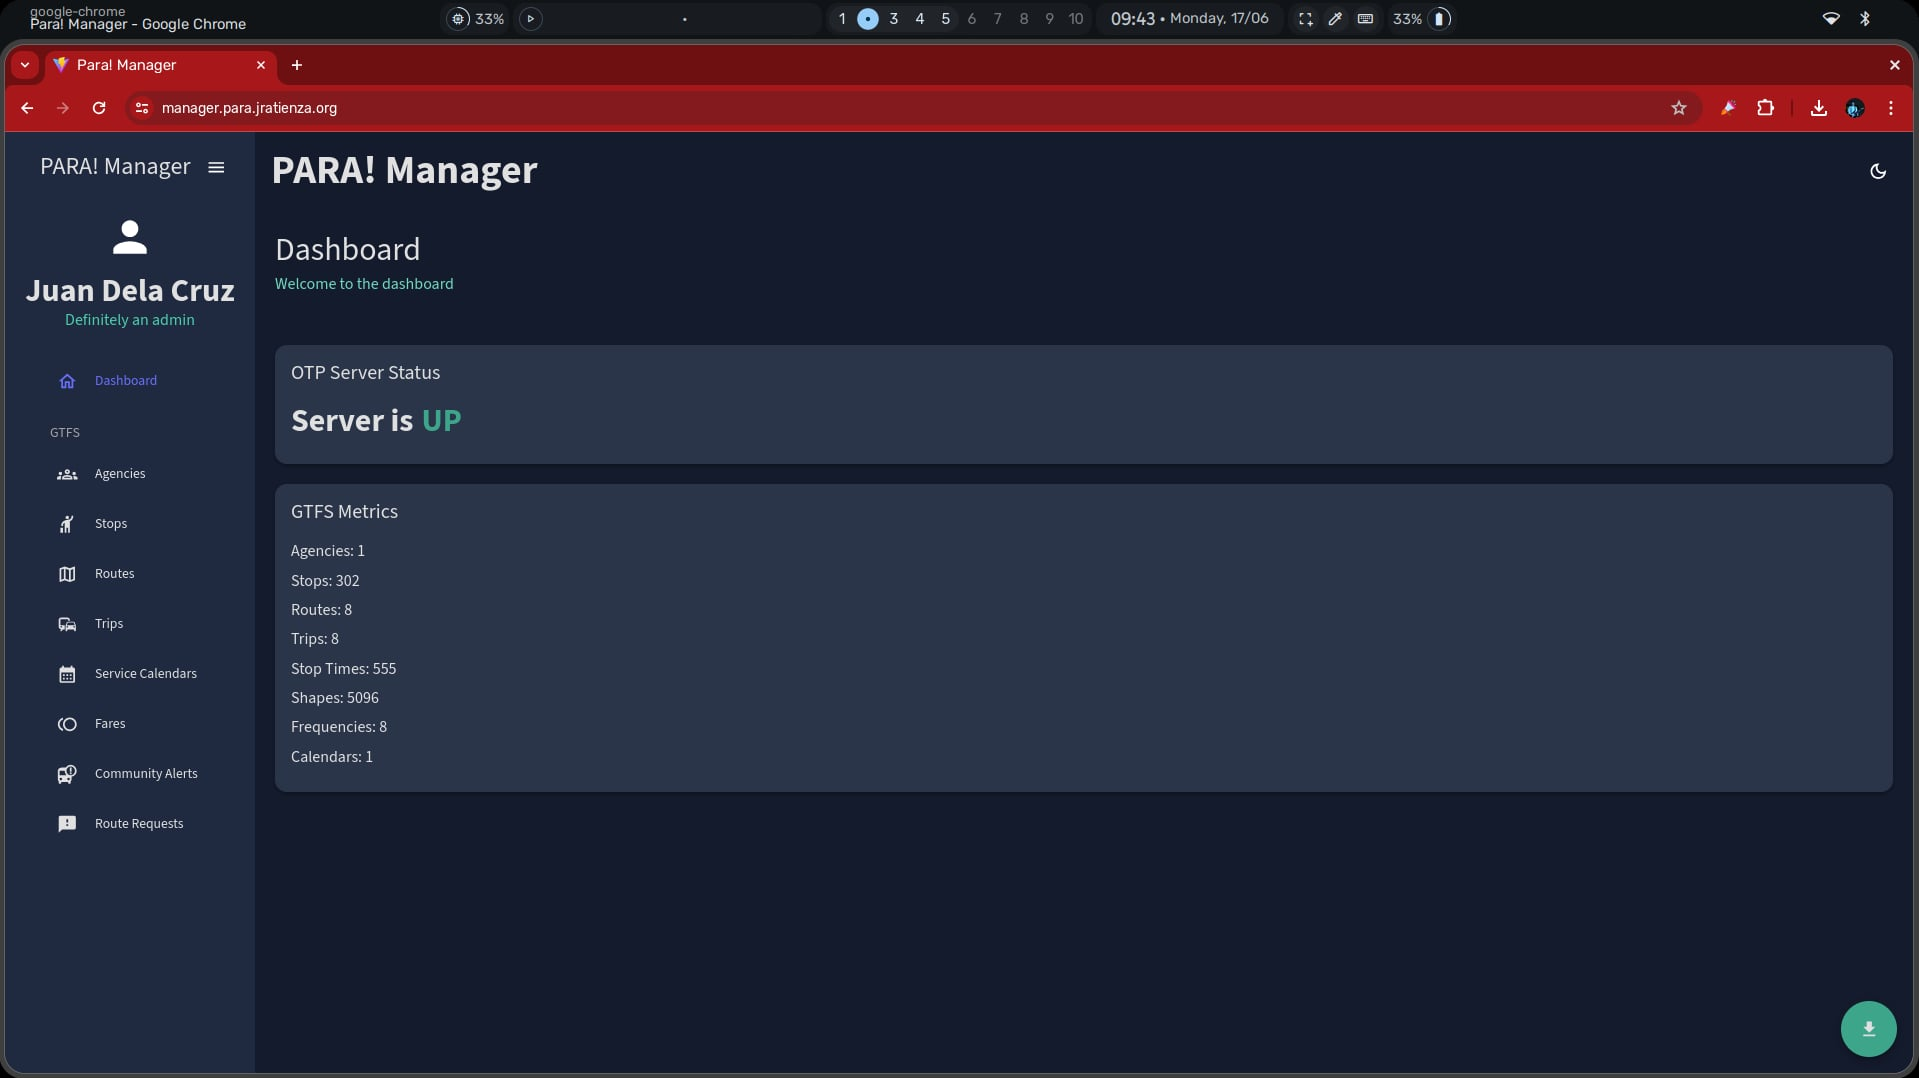
\includegraphics[scale=0.115]{./figures/manager/dashboard.jpeg}
    \caption{PARA! Manager dashboard}
\end{figure}

\item[\textbf{View trips:}] \hfill \\
        Administrators were able to visualize the GTFS data being used by the application. Figure 2 below shows the GTFS data for agency.txt, calendar.txt, frequencies.txt, routes.txt, stops.txt, stop\_times.txt, and trips.txt being consumed and visualized in a modal. 

\begin{figure}[h]
    \centering
        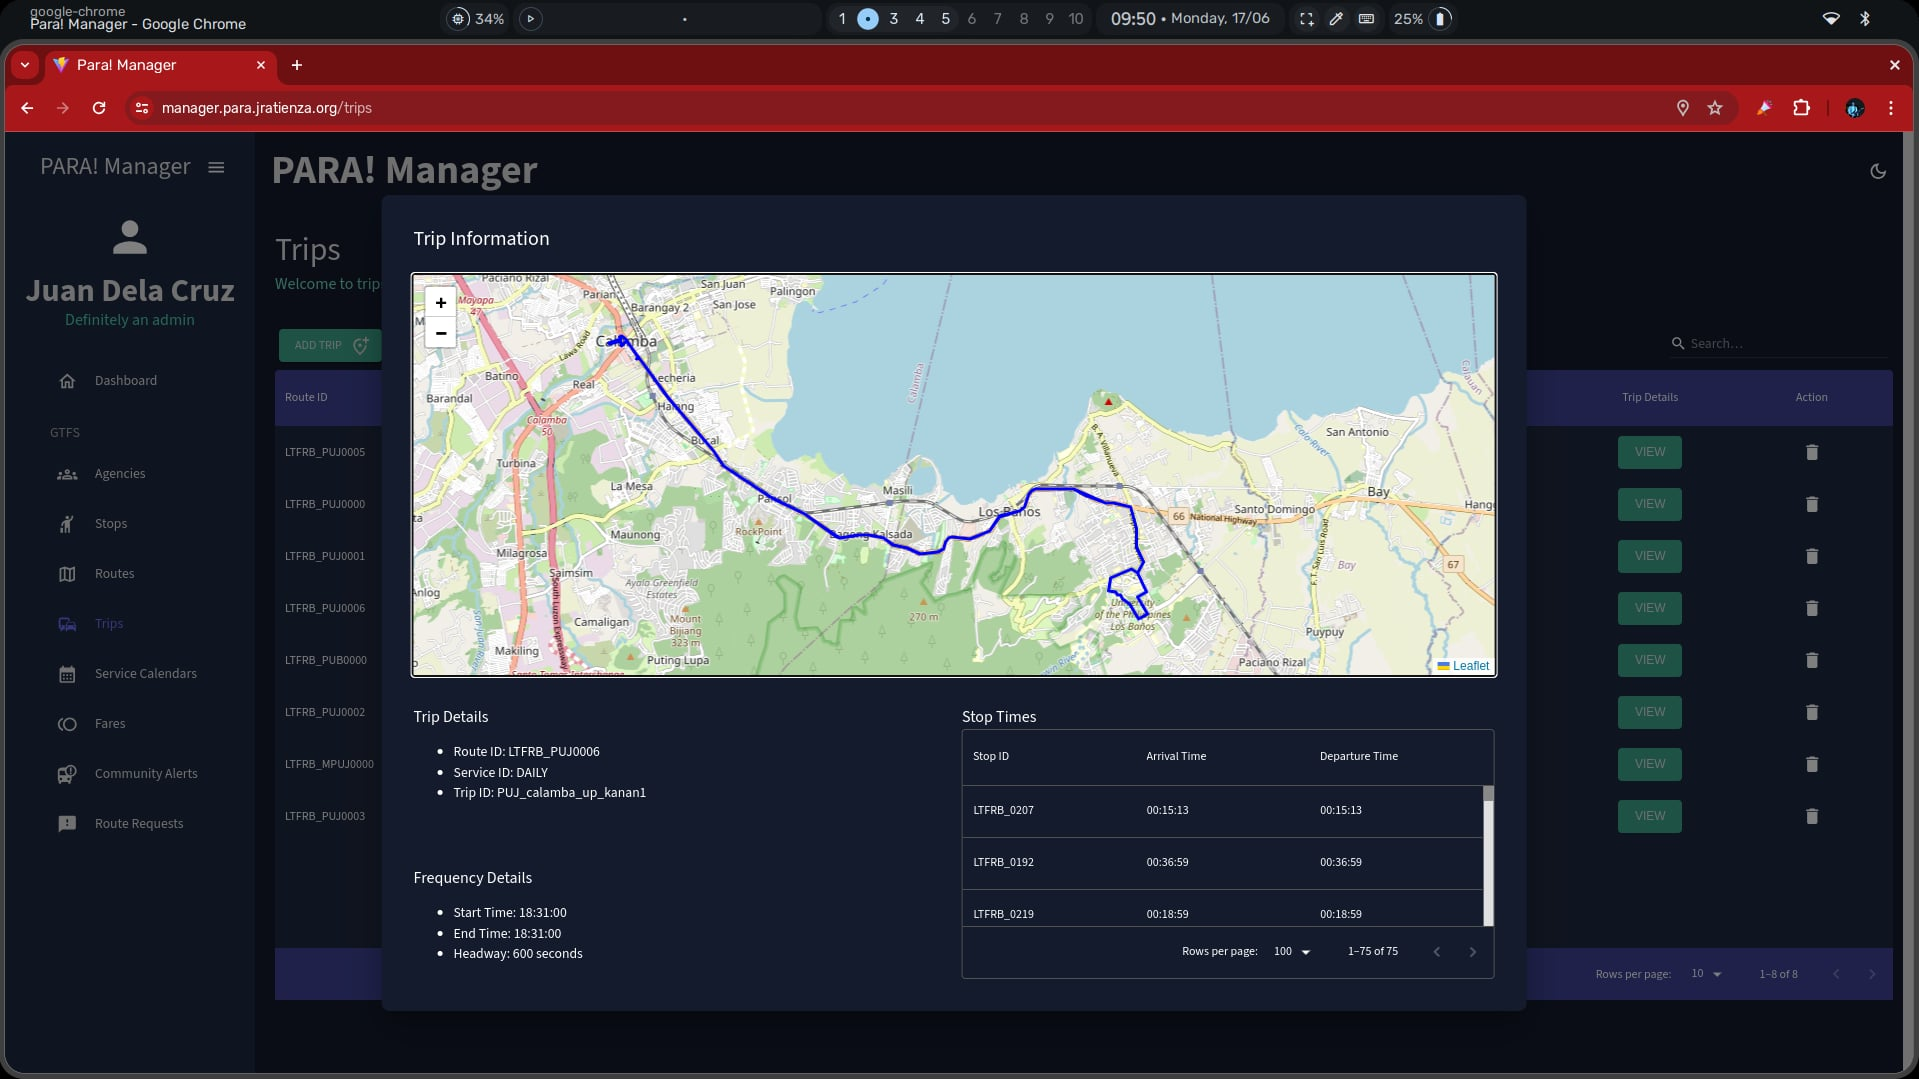
\includegraphics[scale=0.115]{./figures/manager/view trip.jpeg}
    \caption{PARA! Manager trip viewer}
\end{figure}

    \item[\textbf{Interactive GTFS database editor:}] \hfill \\
        Administrators were able to Create, Read, Update, and Delete (CRUD) data to and from the GTFS database that was being consumed by the client-facing application.

\begin{figure}[!h]
    \centering
        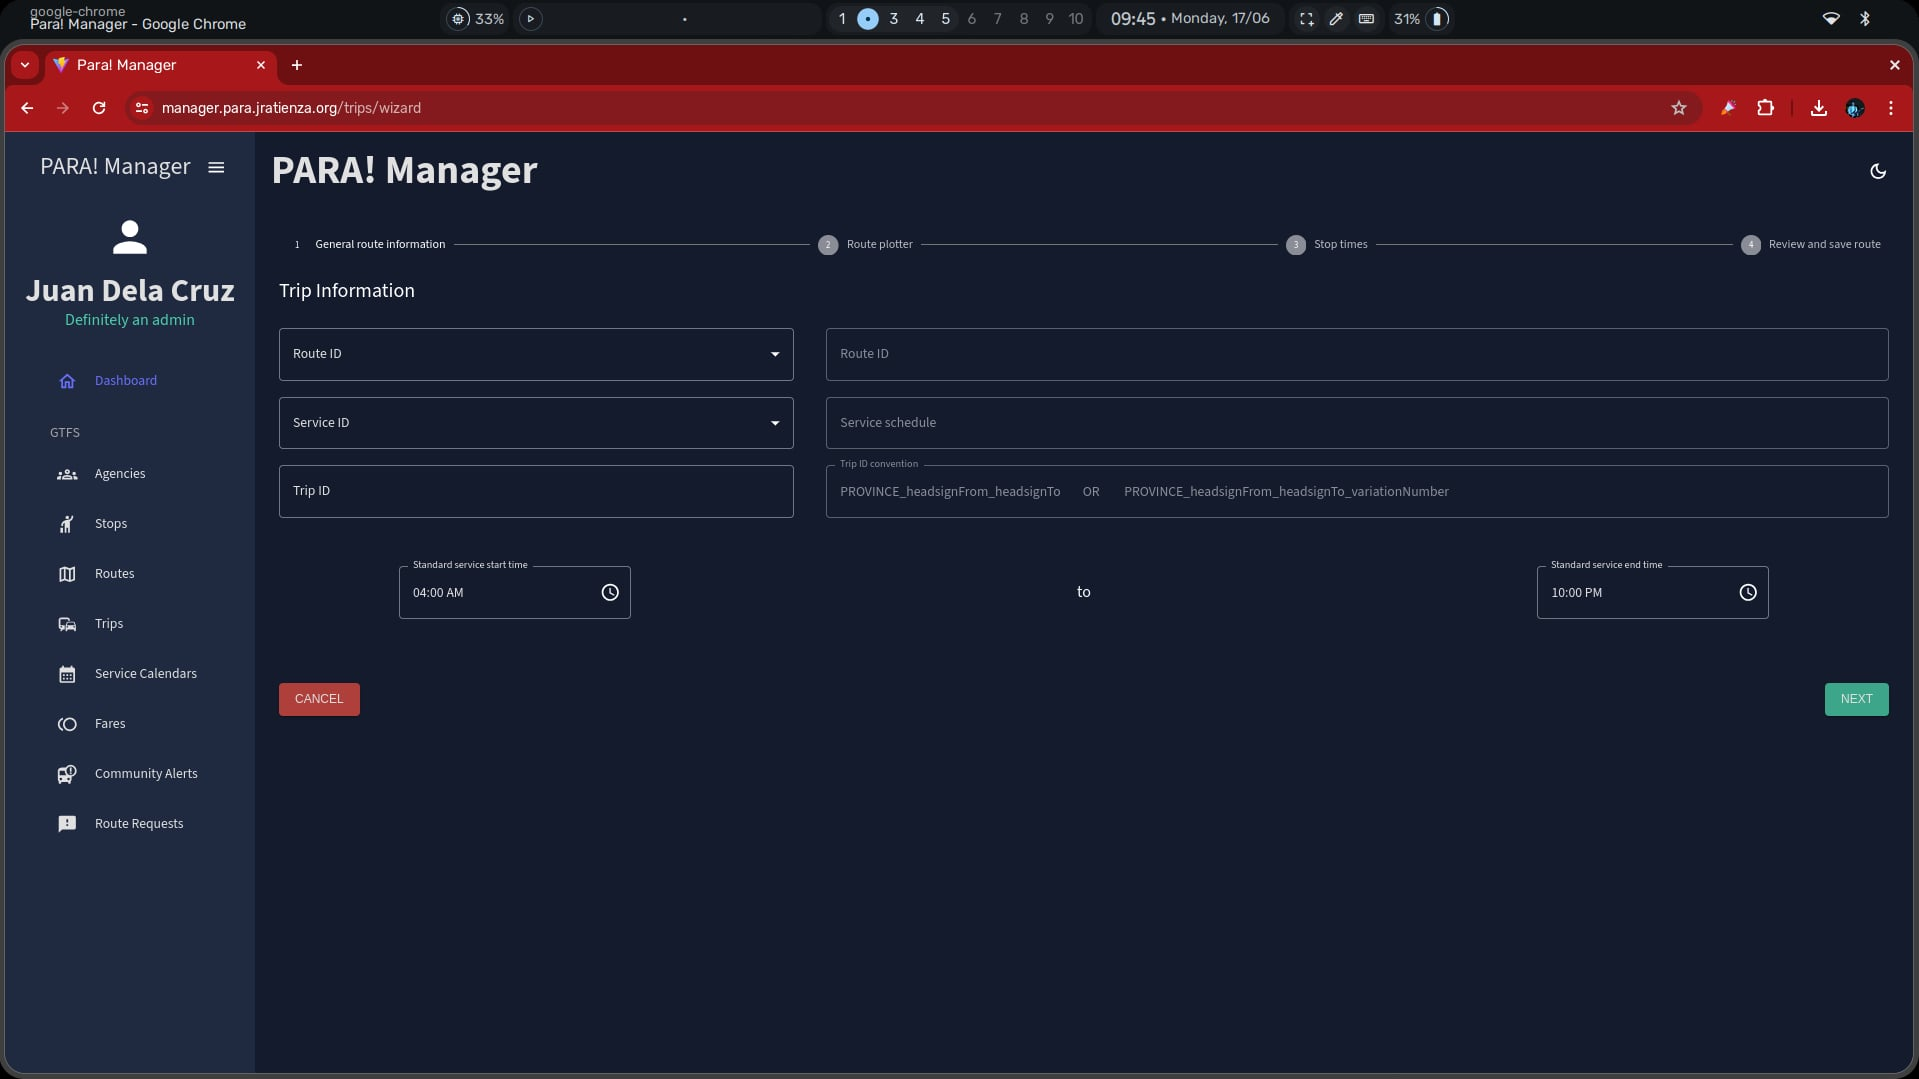
\includegraphics[scale=0.115]{./figures/manager/trip wizard 1.jpeg}
    \caption{PARA! Manager trip wizard (general route information)}
\end{figure}

Figure 3 shows the screen where managers would add general information about the trip.

\begin{figure}[!h]
    \centering
        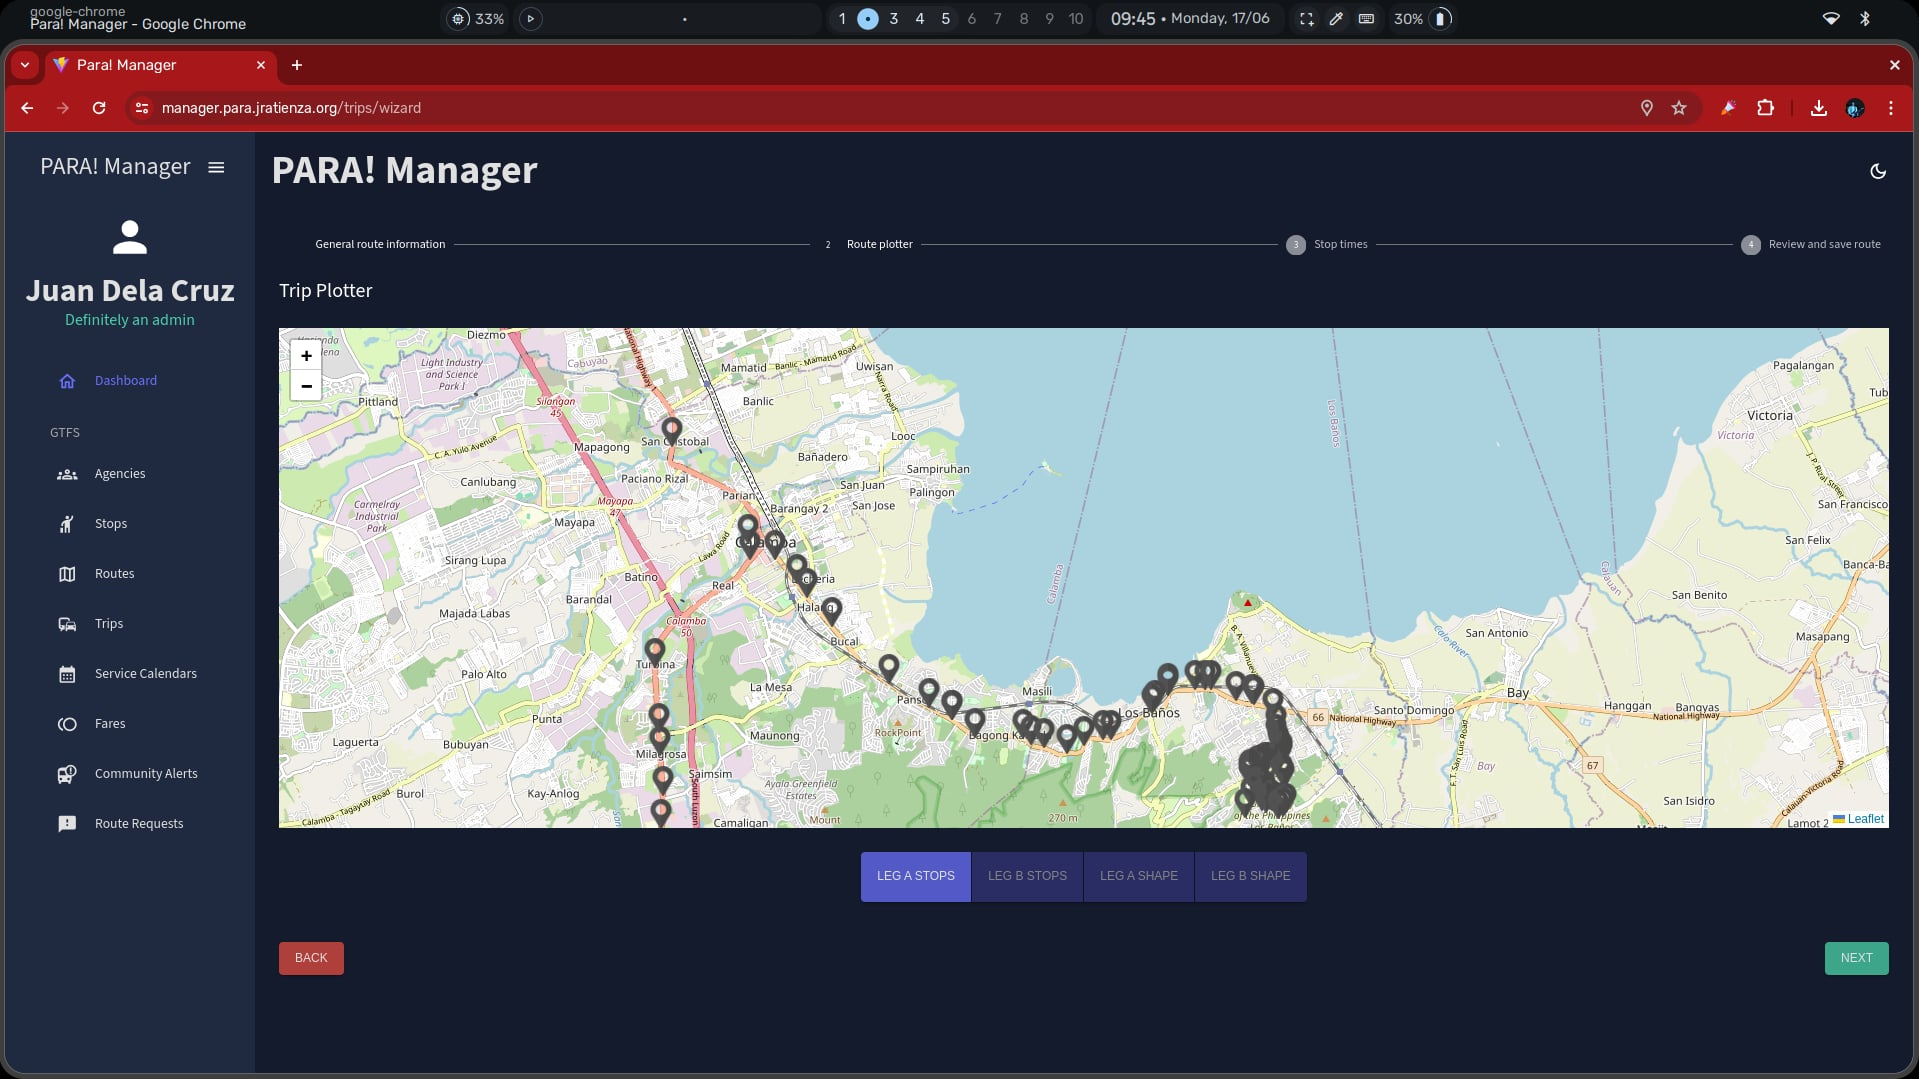
\includegraphics[scale=0.115]{./figures/manager/trip wizard 2.jpeg}
    \caption{PARA! Manager trip wizard (trip plotter)}
\end{figure}

Figure 4 shows the screen where managers would plot a trip's stops and its shape.

\begin{figure}[!h]
    \centering
        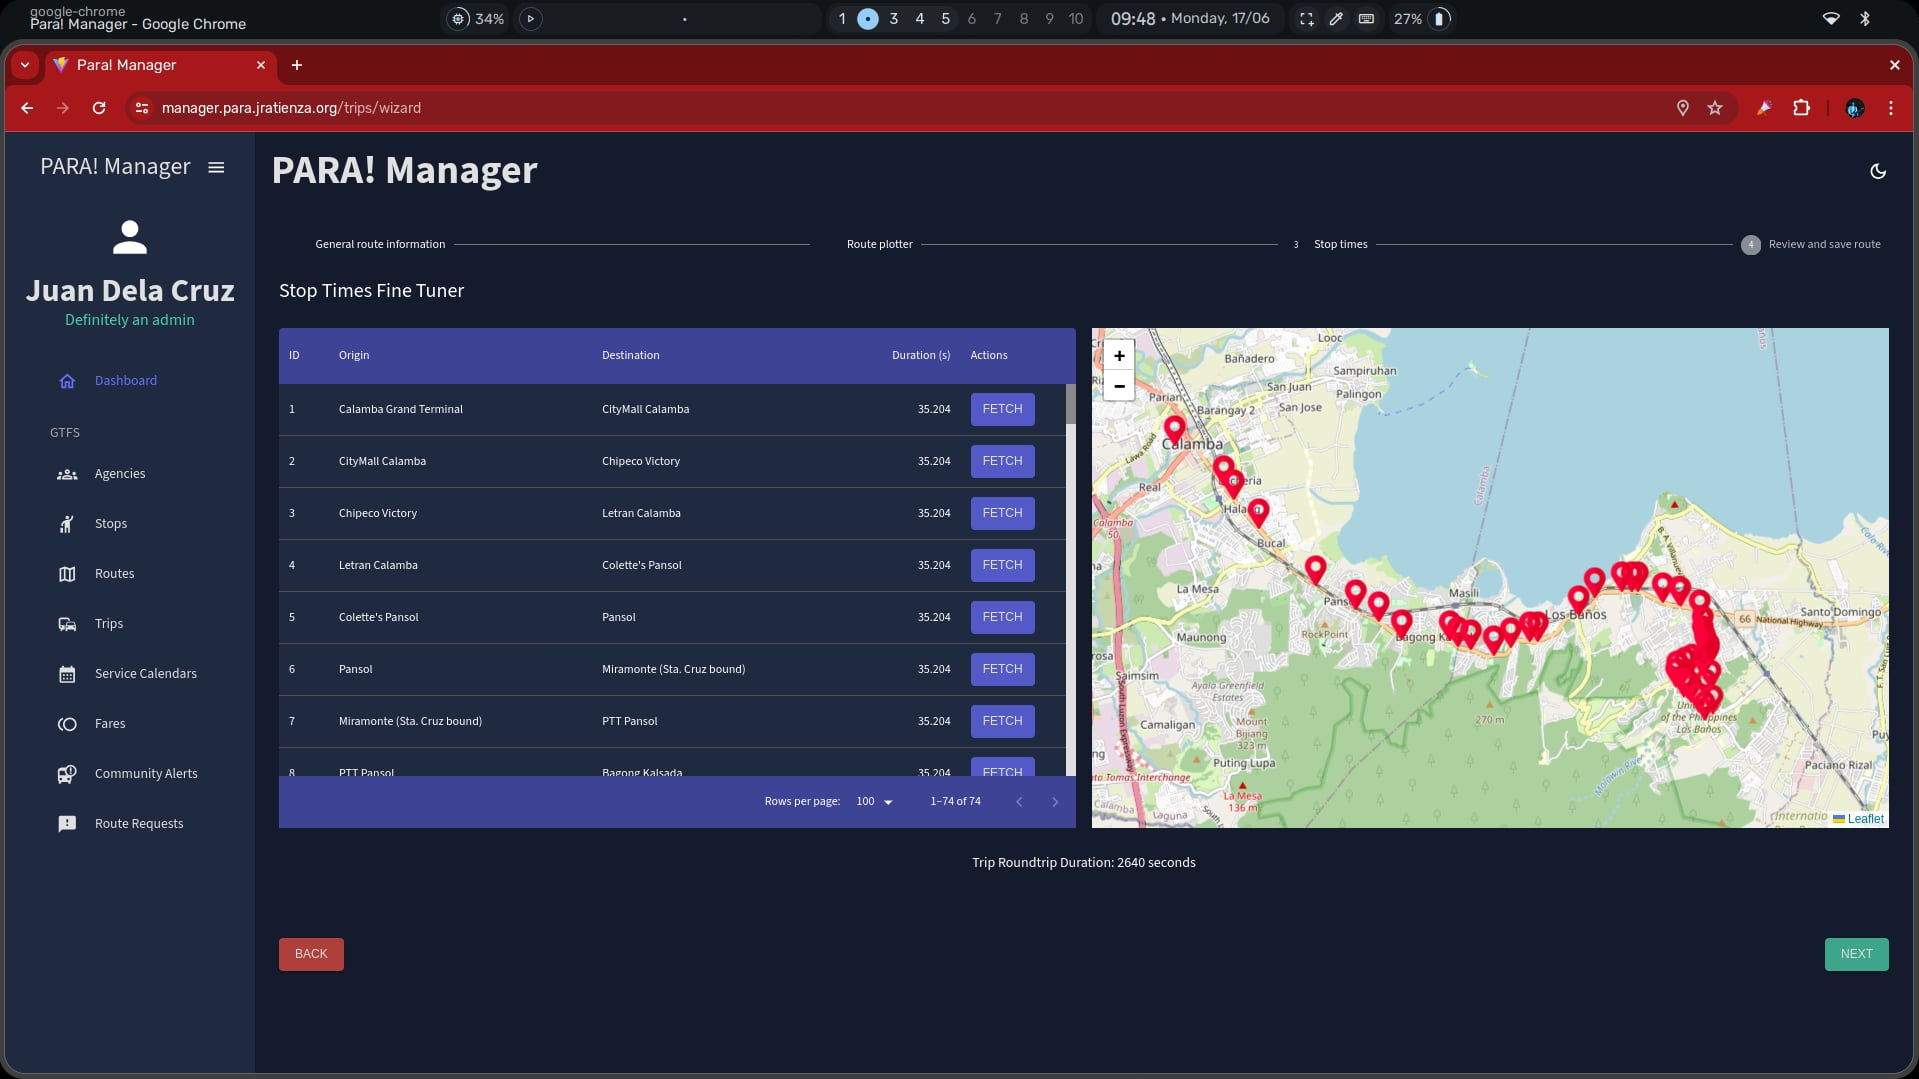
\includegraphics[scale=0.115]{./figures/manager/trip wizard 3.jpeg}
    \caption{PARA! Manager trip wizard (stop times fine tuner)}
\end{figure}

Figure 5 shows the screen where managers would either manually or automatically edit the durations in each segment of the trip. 

\begin{figure}[!h]
    \centering
        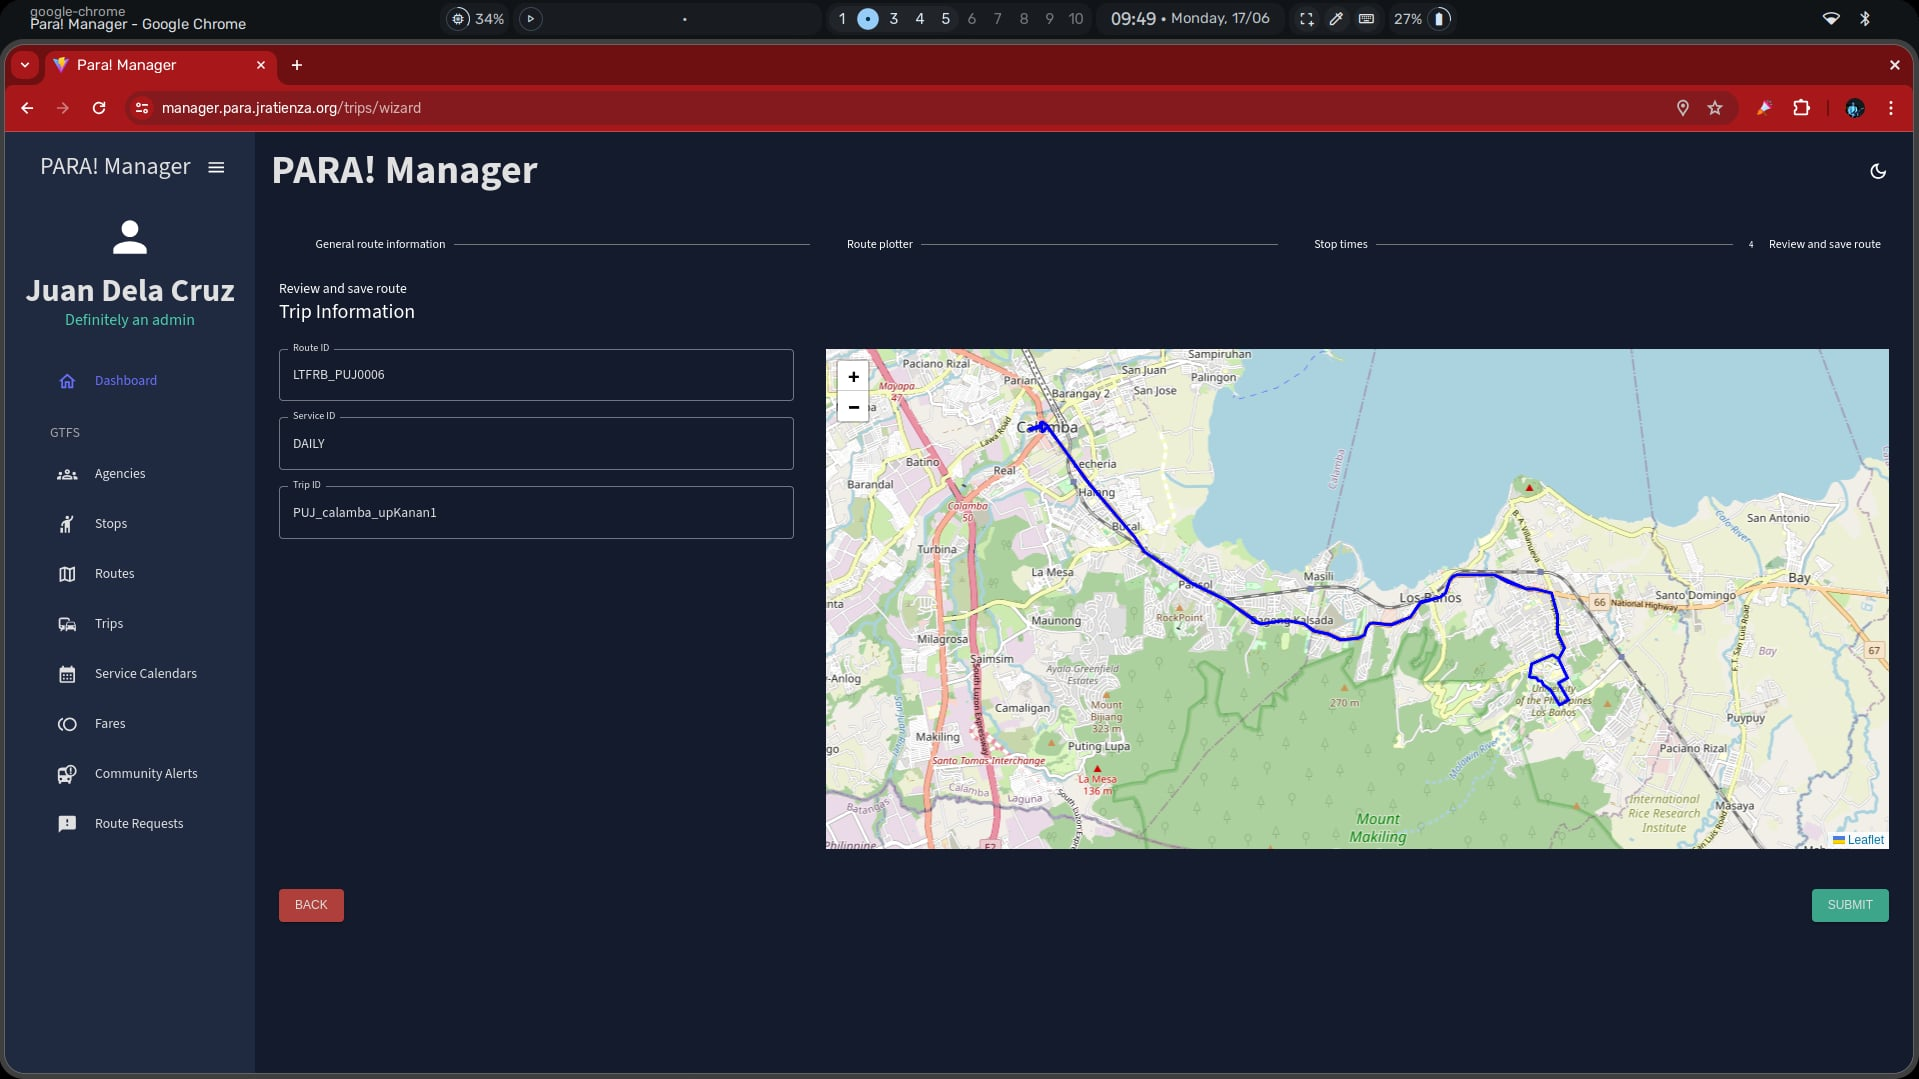
\includegraphics[scale=0.115]{./figures/manager/trip wizard 4.jpeg}
    \caption{PARA! Manager trip wizard (review and save route)}
\end{figure}

Figure 6 shows the screen where managers would review the trip details and its shape before adding it into the database. \hfill \\

    \item[\textbf{View and delete requests:}] \hfill \\
       Administrators were able to view and delete requests made by clients. These requests can be a basis for the creation of new routes or modification of routes in the database.
Figure 7 below shows the screen where managers could view and delete user-submitted route requests.

\begin{figure}[!h]
    \centering
        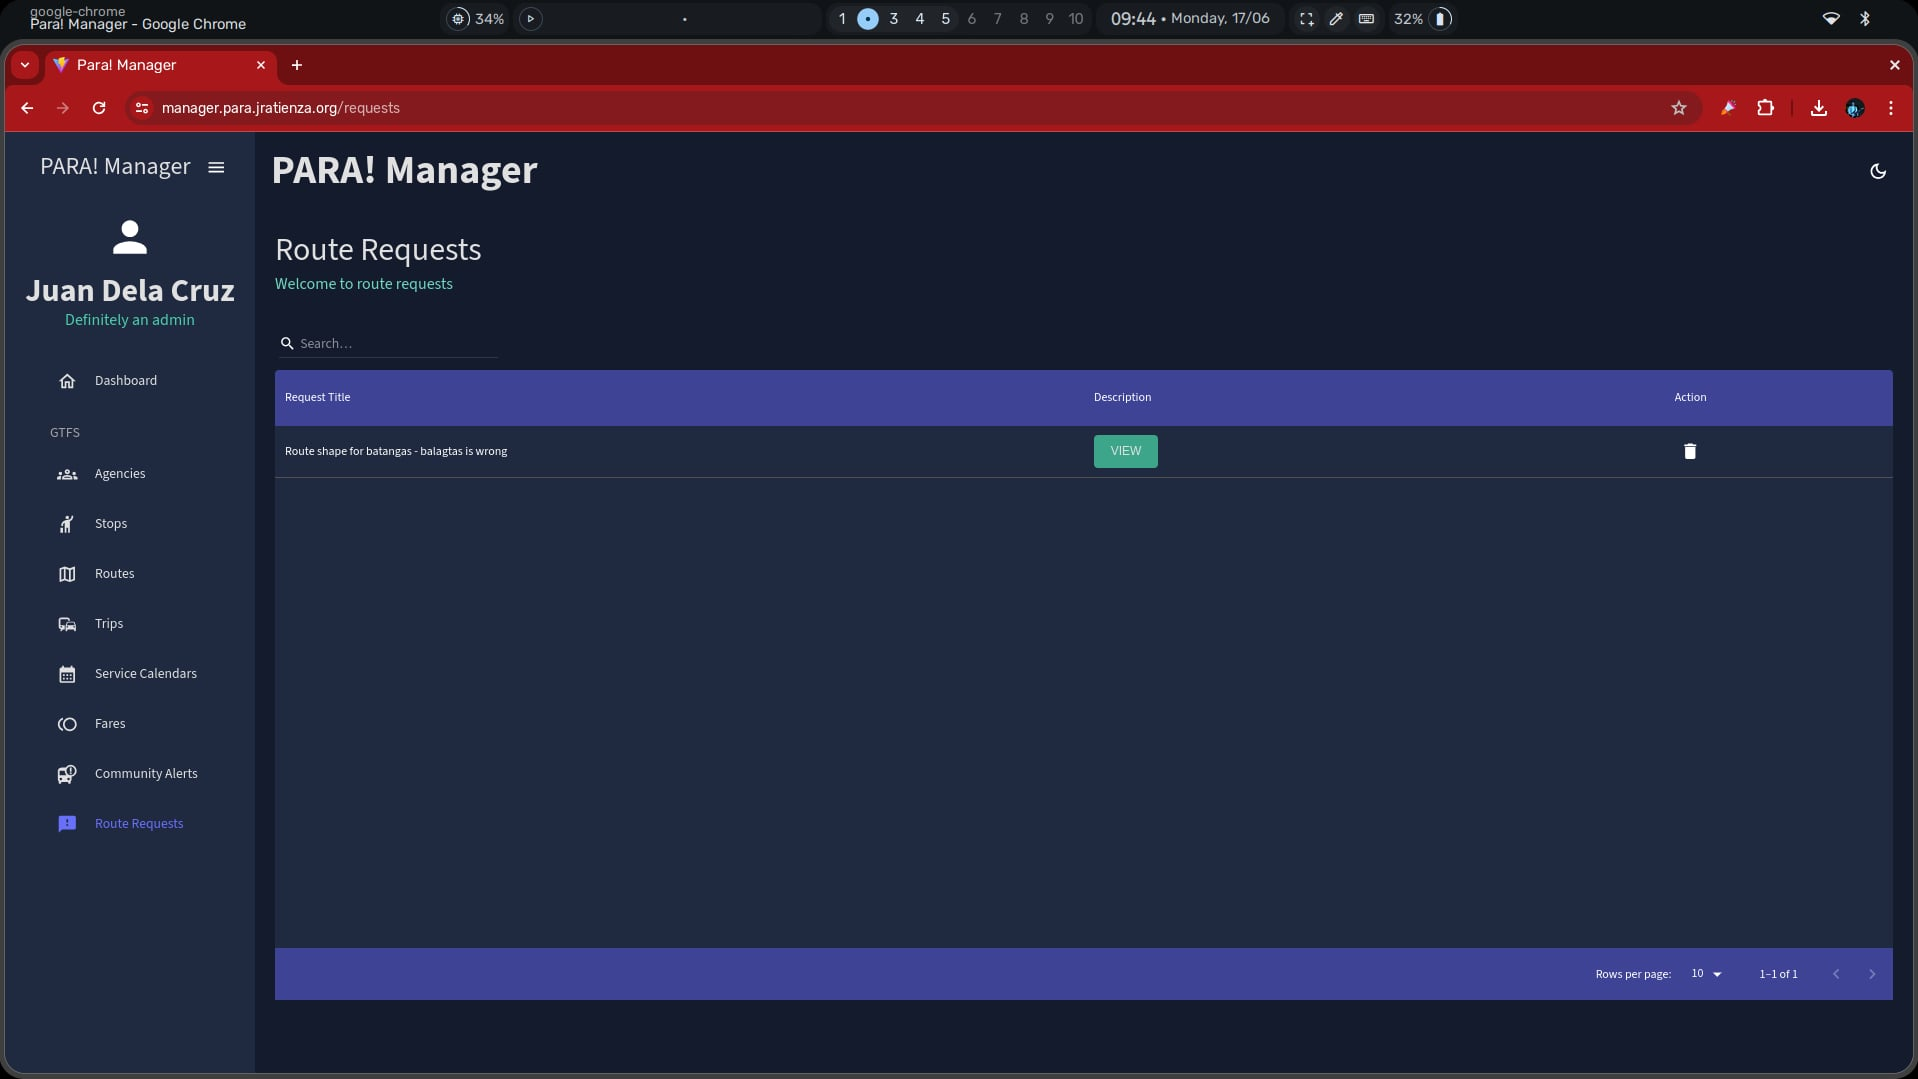
\includegraphics[scale=0.115]{./figures/manager/route request.jpeg}
    \caption{PARA! Manager route requests}
\end{figure}
    
    \item[\textbf{Moderate alerts:}] \hfill \\
       Administrators were able to create, modify, and take down community alerts.
       Figure 8 below shows the screen where managers could add, view, edit, and delete community alerts.
\end{description}

\begin{figure}[!h]
    \centering
        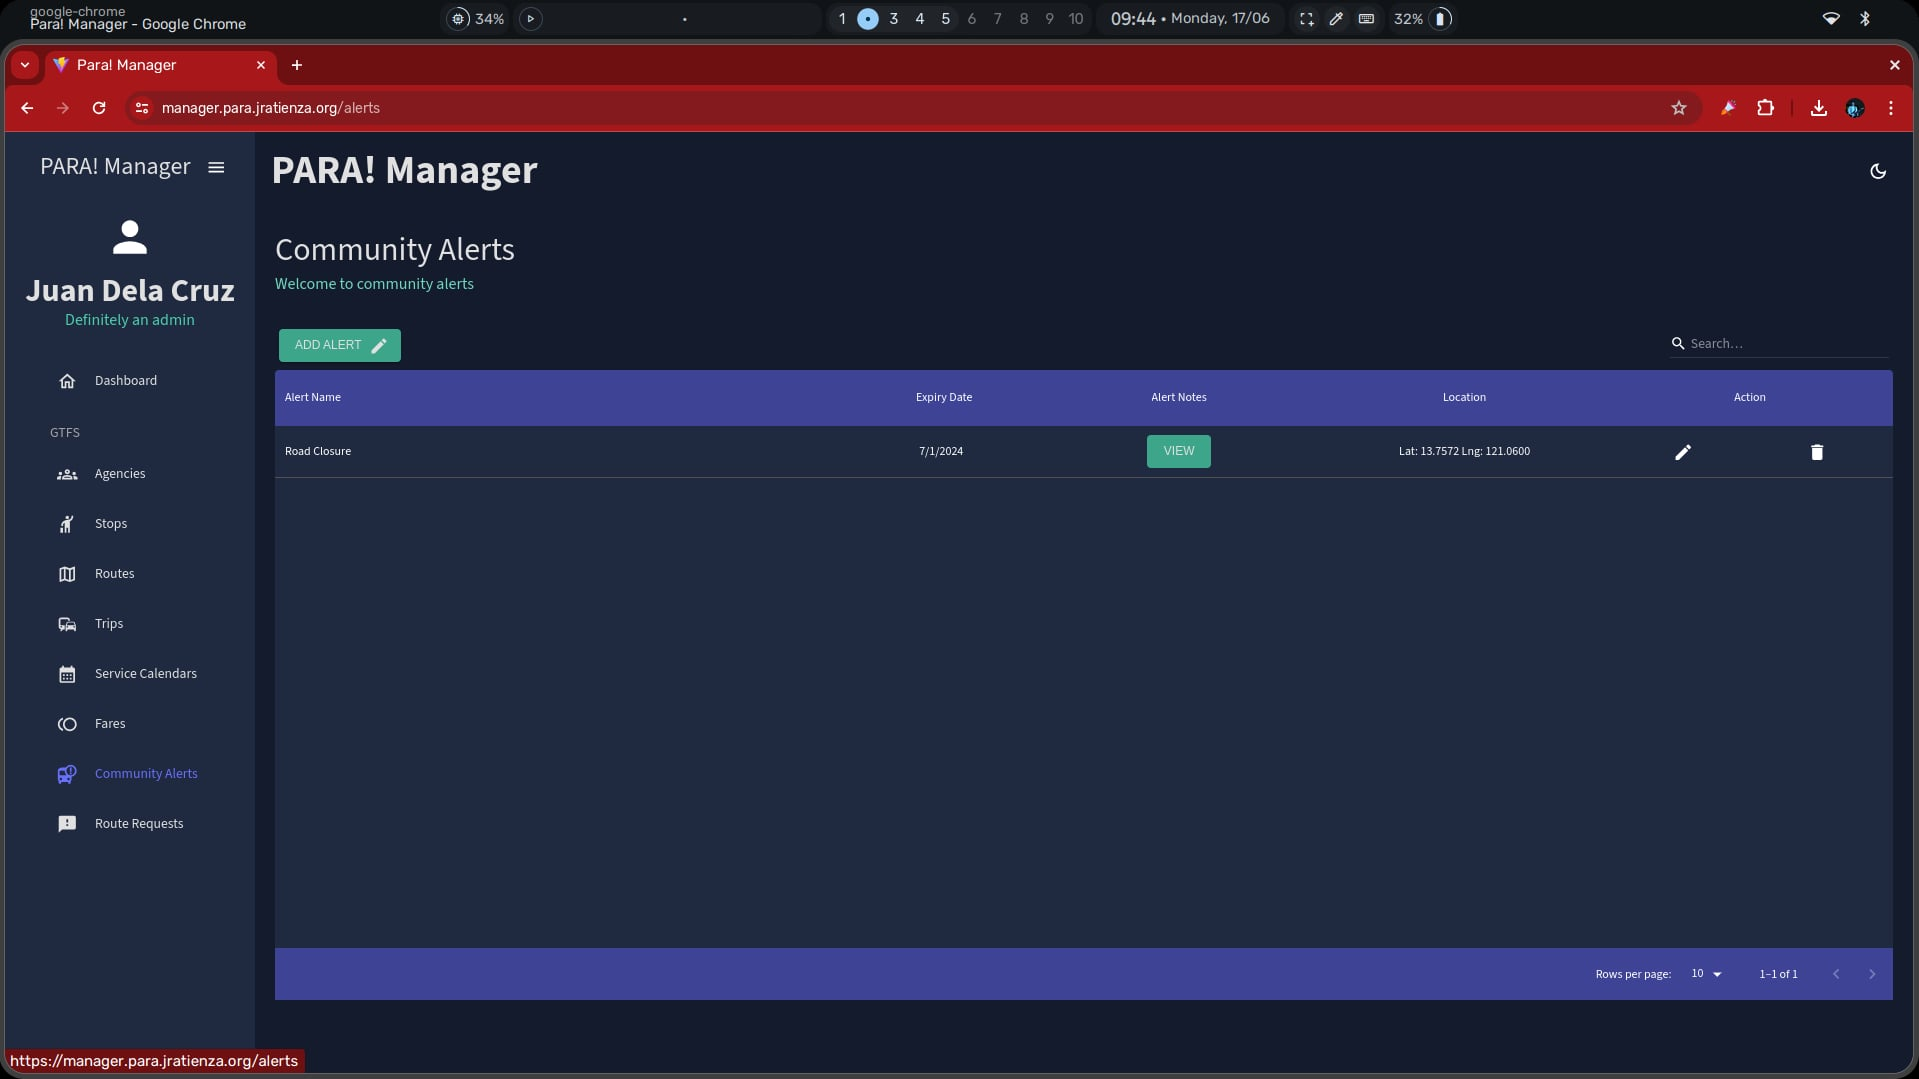
\includegraphics[scale=0.115]{./figures/manager/alerts.jpeg}
    \caption{PARA! Manager trip wizard (review and save route)}
\end{figure}

\subsubsection{\textbf{Client-facing application}}

\begin{description}
%    \item[\textbf{Register:}] \hfill \\
%        Clients are required to register in order to use extended functionalities[*] of the application.

    \item[\textbf{Generate multiple routes:}] \hfill \\
        Multiple routes are generated given an origin and destination. Appropriate fare pricing based on LTFRB's specification, along with per-leg and overall trip duration, will also be displayed.
Figure 9 on the next page shows the screen where multiple routes are generated given an input of an origin and destination.
The overall duration and fare is displayed on the top-left section of the DraggableScrollableSheet Widget while the duration and fare for each leg are displayed on the rightmost part of each itinerary leg entry (see Appendices I-IV for the fare computation formulae and sample fare matrices (as of October 8, 2023) provided by LTFRB RO-4A).
Each route is color-coded through a custom random color generator function. In the figure, there are only two colors, teal and dandelion, which could be subtly seen due to the overlap in the route.
The figure also shows a red "warning" icon which when tapped, shows details of a user- or manager-generated community alert.

\newpage

\begin{figure}[h]
    \centering
        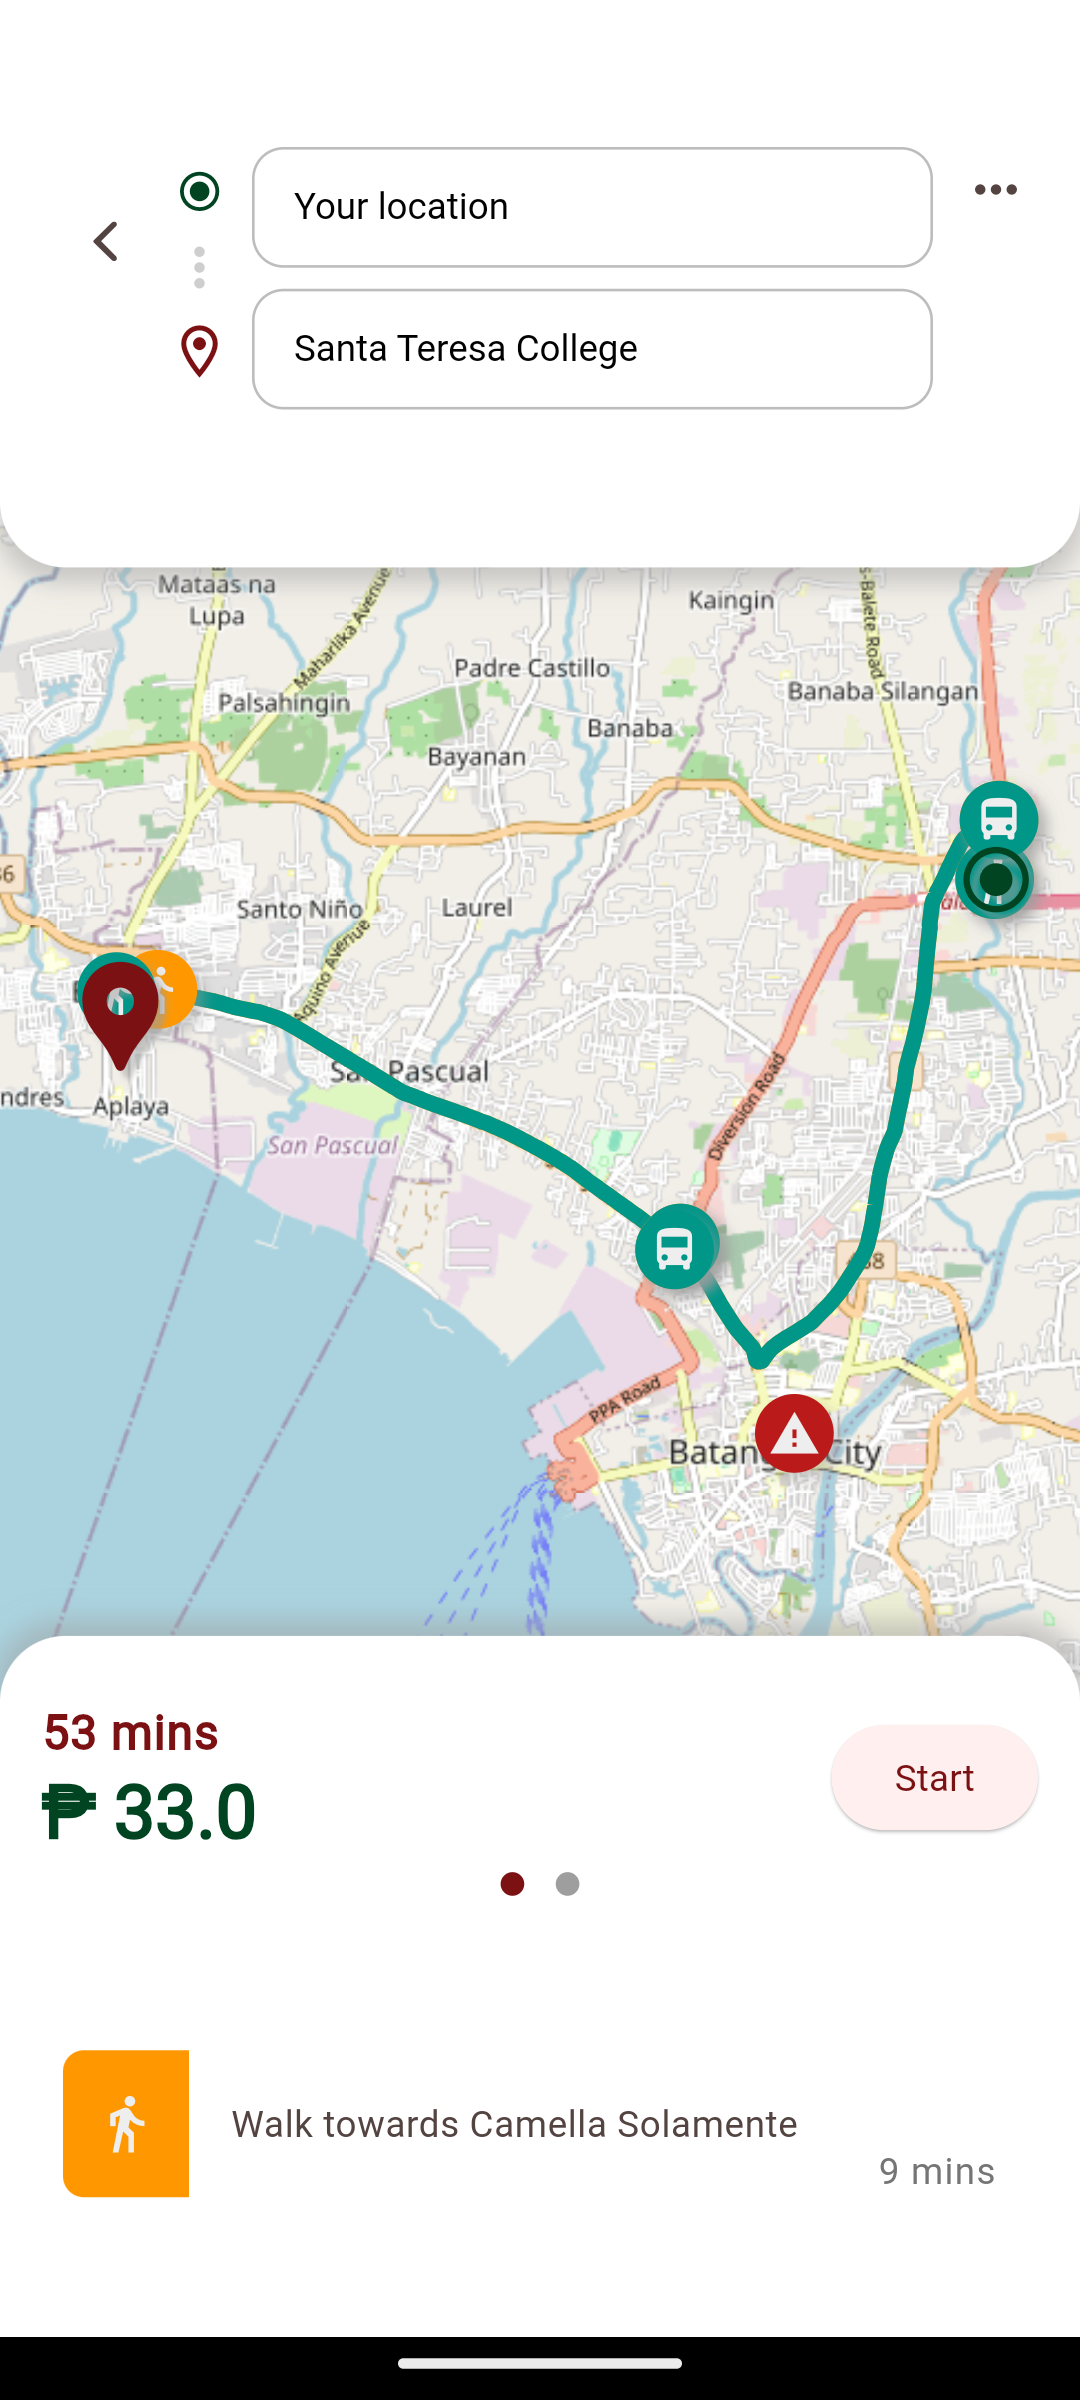
\includegraphics[scale=0.1]{./figures/client/multiple route.png}
    \caption{PARA! Client (generated multiple routes)}
\end{figure}

    \item[\textbf{Generate public alerts:}] \hfill \\
        Clients generated public alerts, such as vehicular accidents, to alert commuters. Users were also able to set an expiry date (maximum of 30 days) which set the Time To Live (TTL) of the alert in the database for automatic cleanup.
        Figure 10 below shows the add community alert function which could be accessed through the "plus" icon in the bottom nav bar (Figure 11) or through the floating action button within the community alerts screen, which could be accessed through the Home Menu (Figure 12).

\begin{figure}[!h]
    \centering
        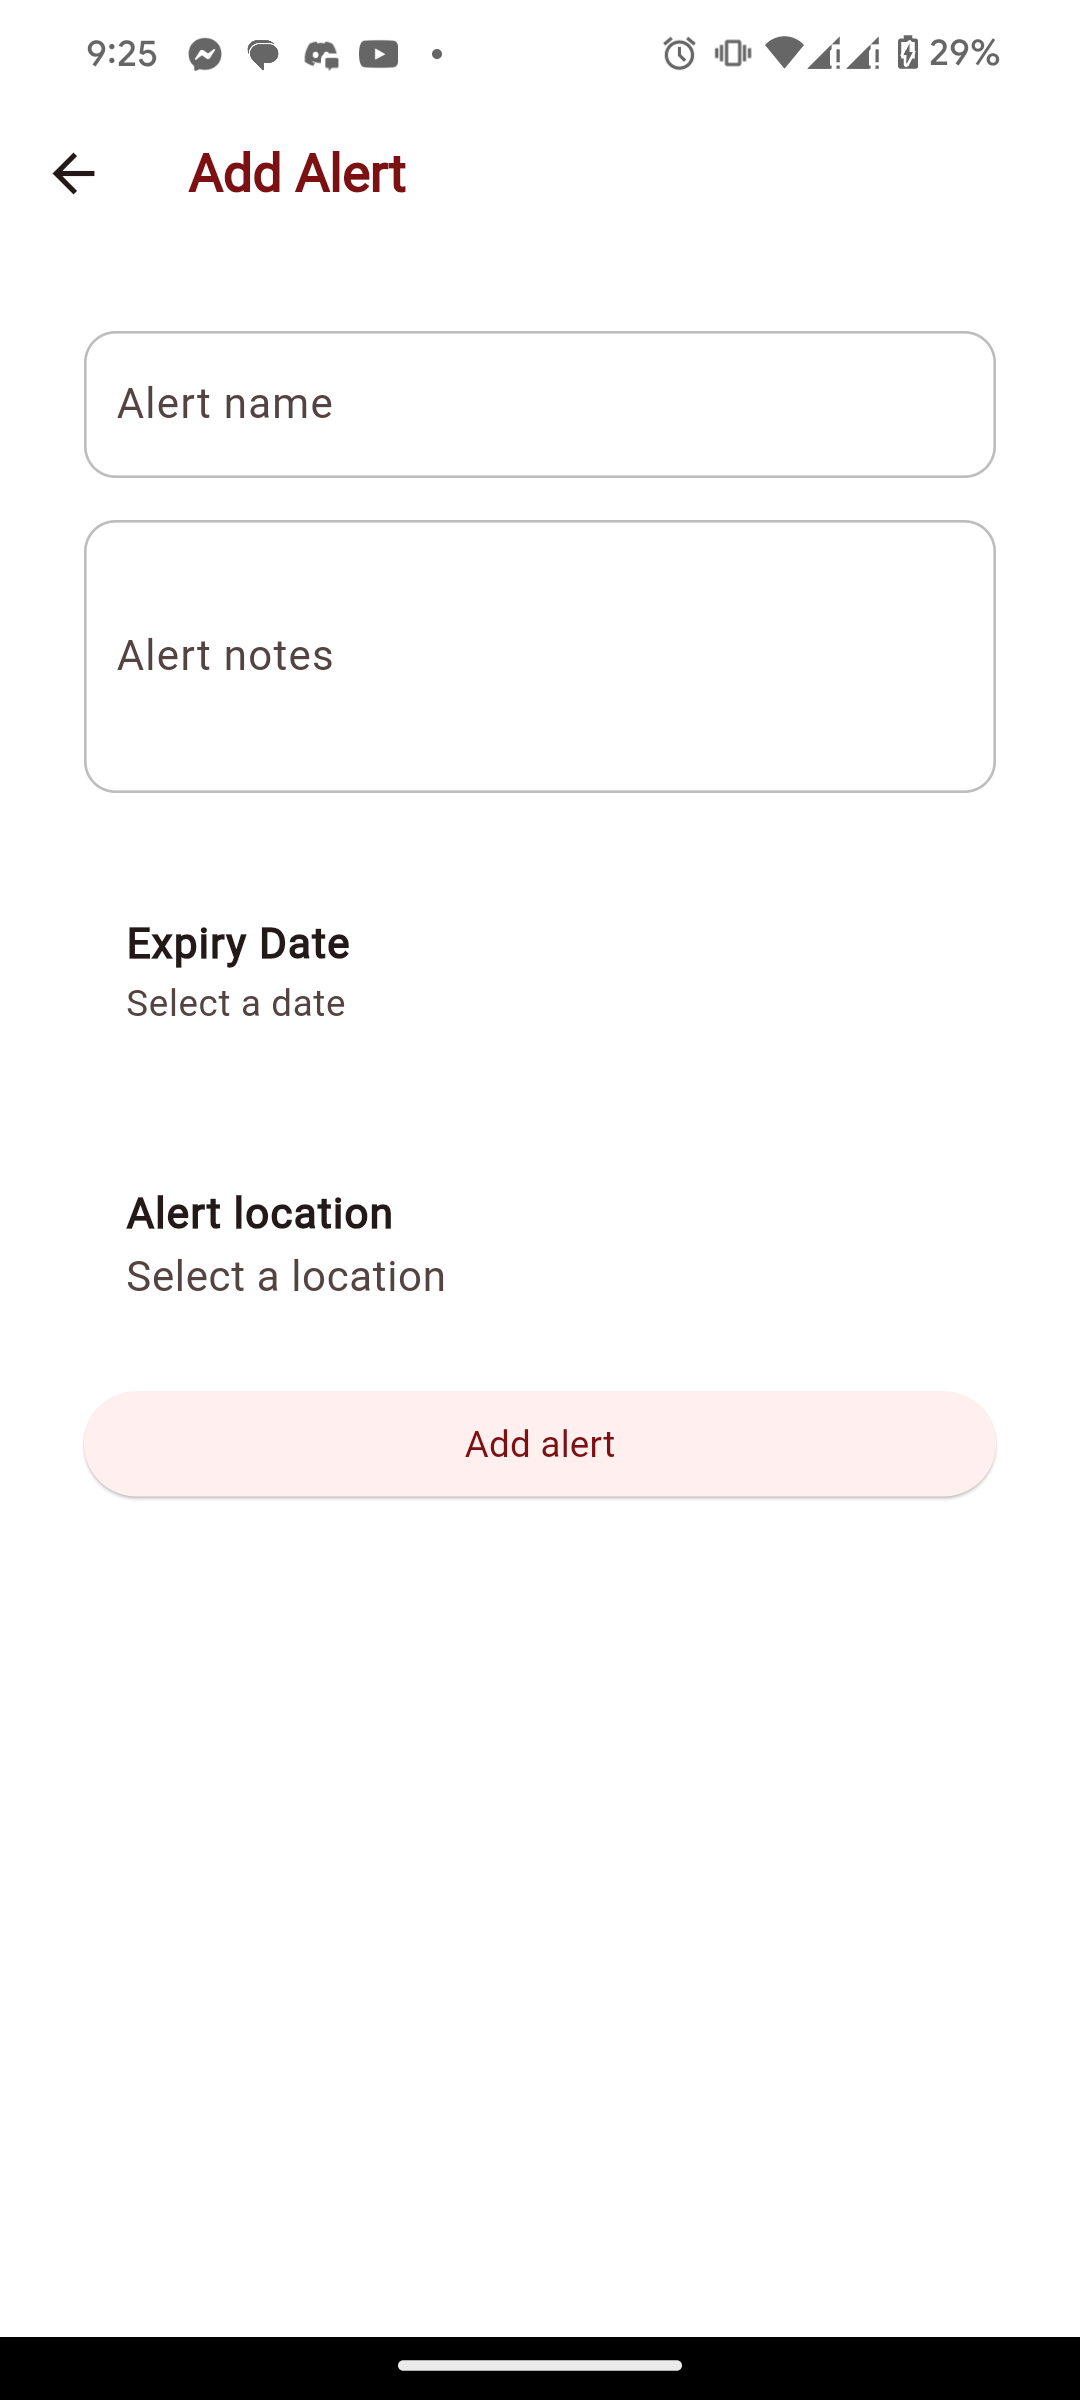
\includegraphics[scale=0.1]{./figures/client/add alert.png}
    \caption{PARA! Client add community alert}
\end{figure}

\begin{figure}[!h]
    \centering
        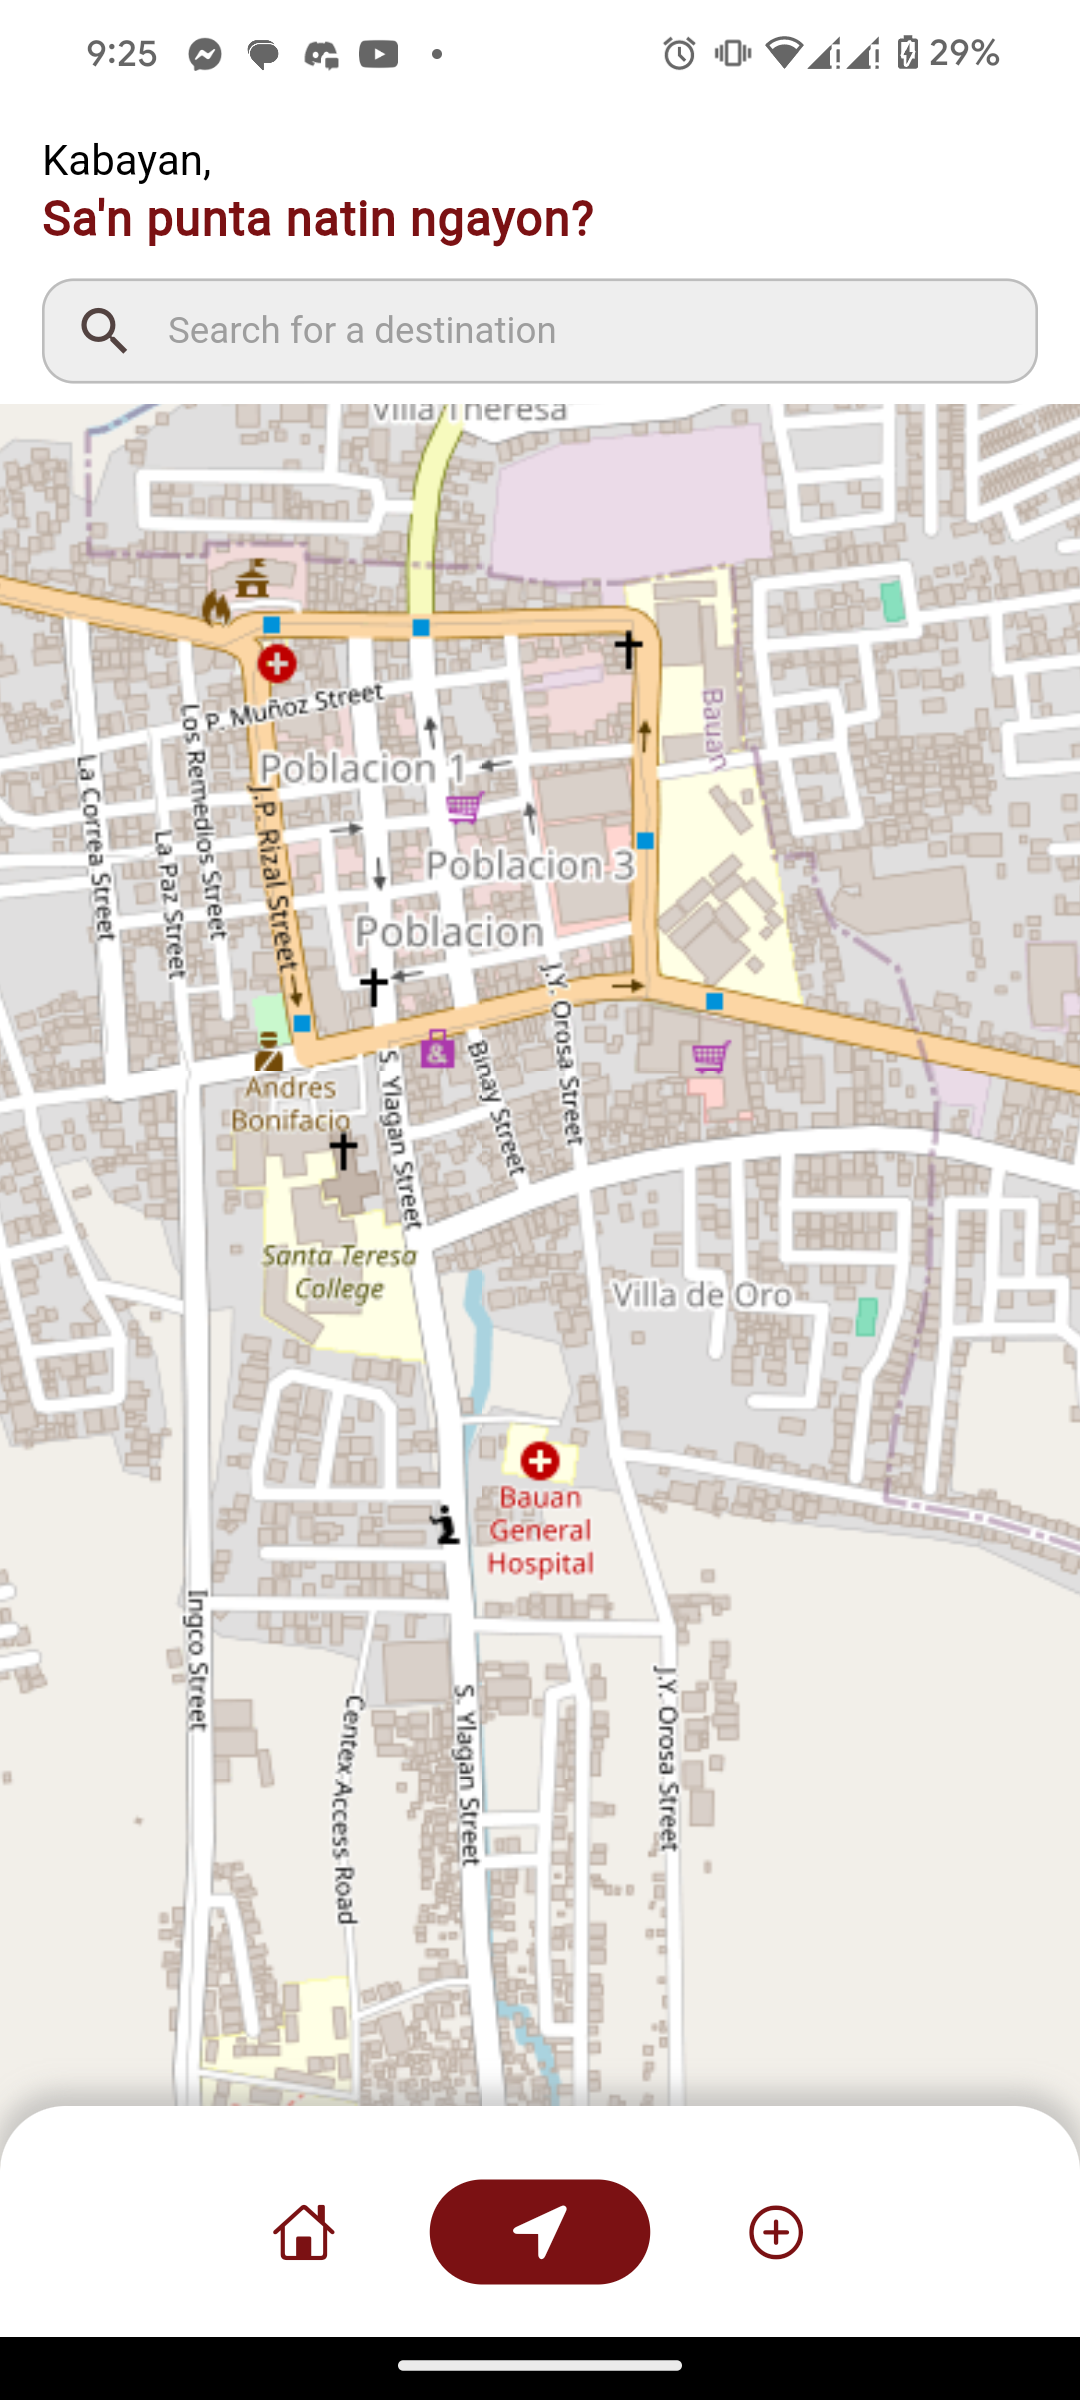
\includegraphics[scale=0.1]{./figures/client/welcome.png}
    \caption{PARA! Client initial screen}
\end{figure}

\begin{figure}[!h]
    \centering
        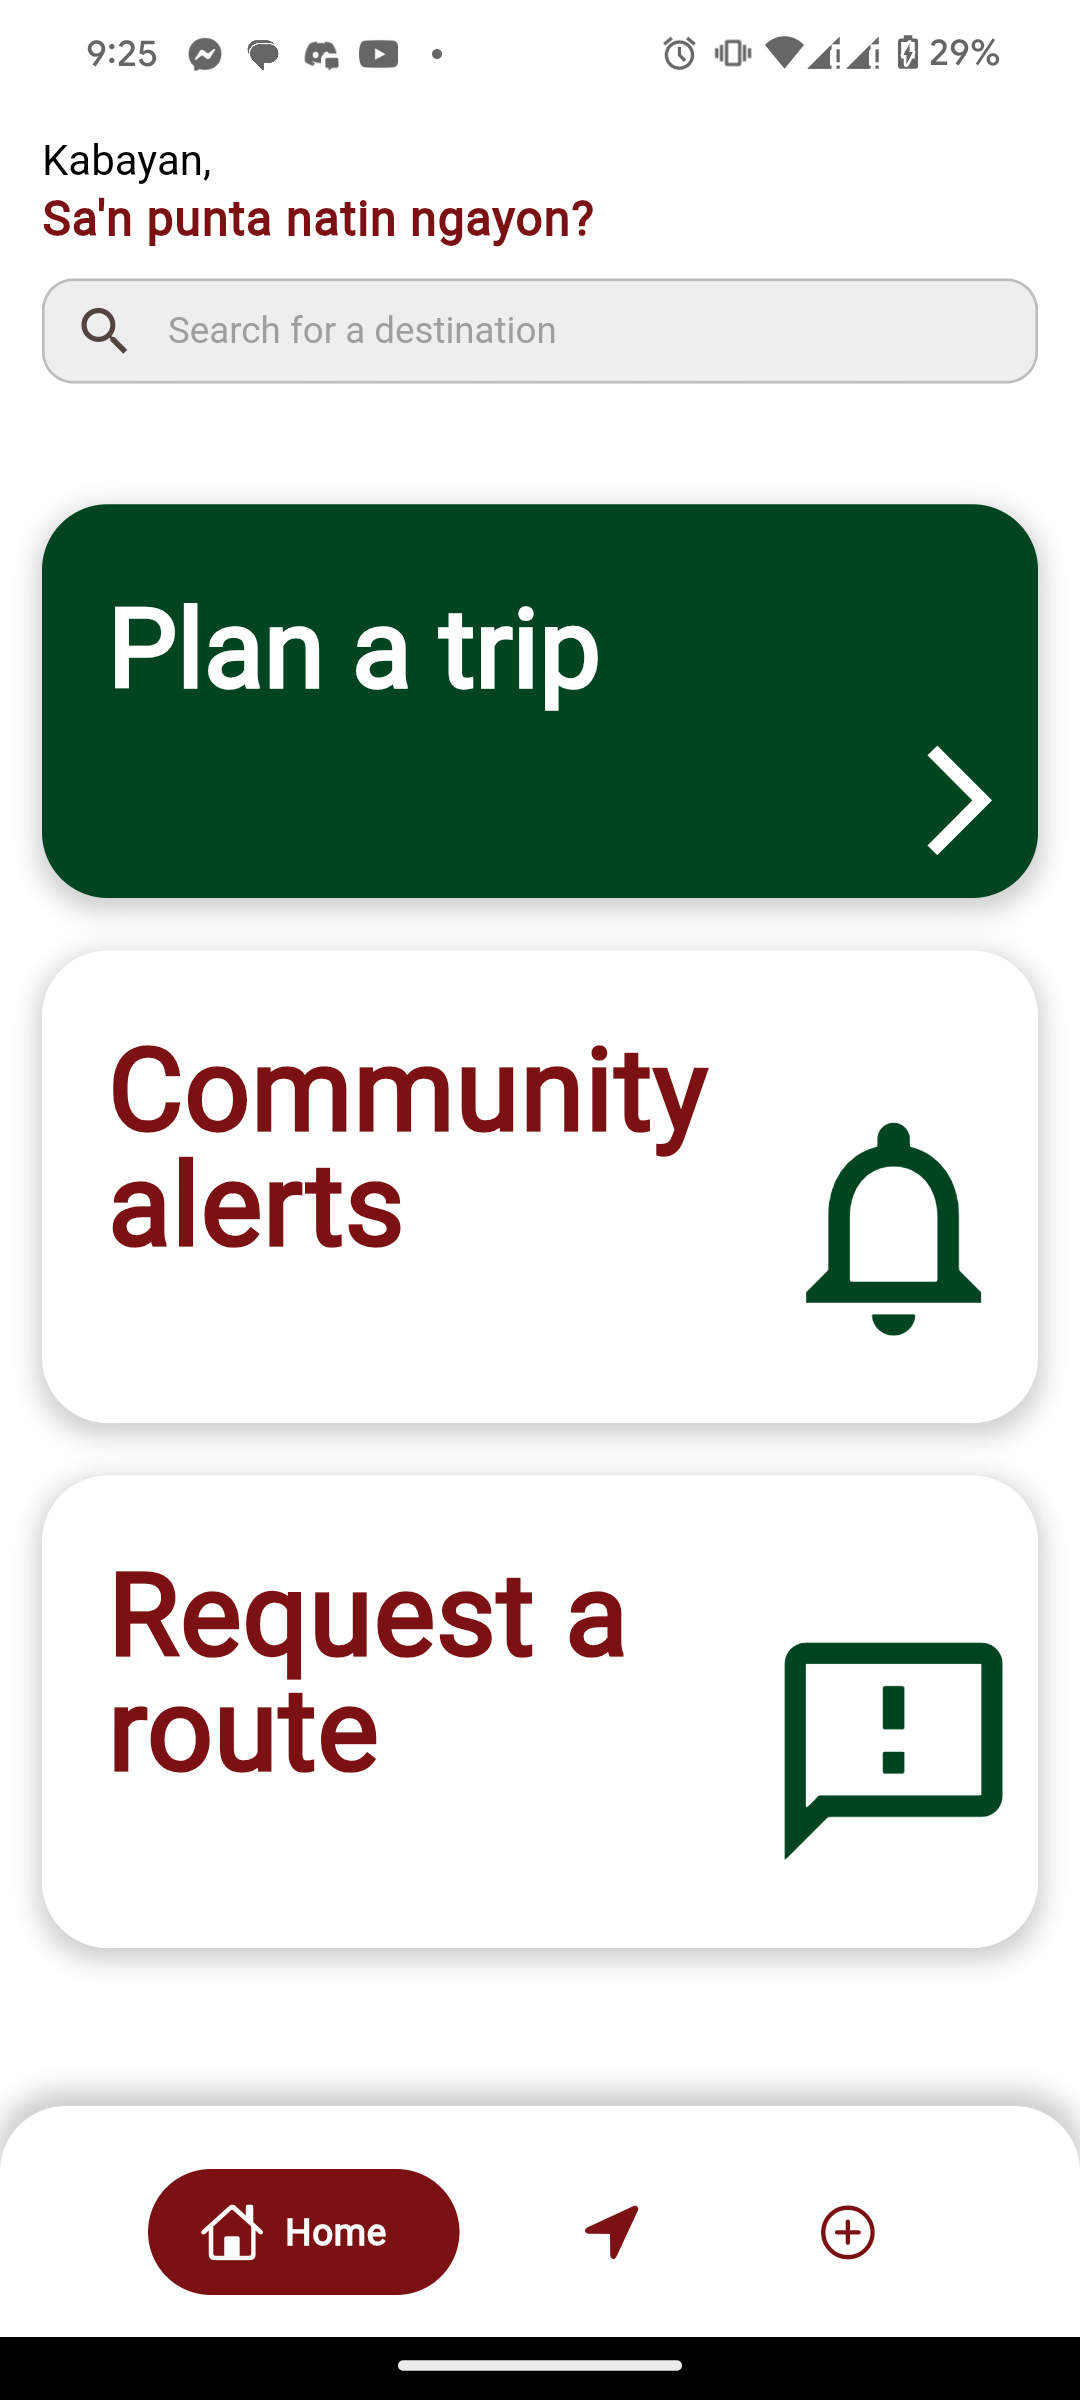
\includegraphics[scale=0.1]{./figures/client/home menu.png}
    \caption{PARA! Client home menu}
\end{figure}

% \item[\textbf{Add Routes*:}] \hfill \\
   %     Registered clients can add routes or request changes in a particular route. A prompt asking for GTFS-ready information will be used.
\end{description}

\subsection{User Evaluation}
For the usability and user experience aspect, the client-facing application was tested by students residing in Batangas Province, transport operators, and transport enthusiasts willing to take part in the study. For evaluators using an Android device, the APK of the application were provided.
The management application was tested by a representative from LTO Calapan.
%For iPhone users, Expo Go will be used to communicate with the Expo server that will be ran by the proponent.

The usability and user experience aspect were measured using the Usefulness, Satisfaction, and Ease of Use (USE) Questionnaire~\cite{Lund01}, a 7-point likert scale. 

%For the maintainability aspect as denoted in objective 6, the application is tested by senior BS Computer Science students, the UPLB ICS Faculty, and other IT experts. The GitHub repository used in the development process of the application will be provided for them. A software complexity report generated by the npm package `complexity-report' will also be provided.

%In measuring the maintainability of the source code, a questionnaire will be used to measure the estimated rebuild value, percentage of redundant code, lines of code per unit, cyclomatic complexity per unit (provided by the report), number of parameters per unit, and number of incoming calls per module.
%The metrics would be used to evaluate the volume, duplication, unit size, unit complexity, unit interfacing, and module coupling properties that would be mapped to the ISO/IEC 9126 metric.
%Additional information in the form of remarks will also be in the questionnaire which will be subjected to qualitative assessment.

% RESULTS AND DISCUSSION
\section{Results and Discussion}
A total of 21 individuals participated in the client-facing app evaluation while there was only a single certified tester for the management application. The interpretation for the 7-point Likert scale is the following:

\begin{description}
    \item 1 --- Strongly disagree
    \item 2 --- Disagree
    \item 3 --- Somewhat disagree
    \item 4 --- Neutral
    \item 5 --- Somewhat agree
    \item 6 --- Agree
    \item 7 --- Strongly agree.
\end{description}

\subsection{Management application}
\begin{figure}[h]
    \centering
        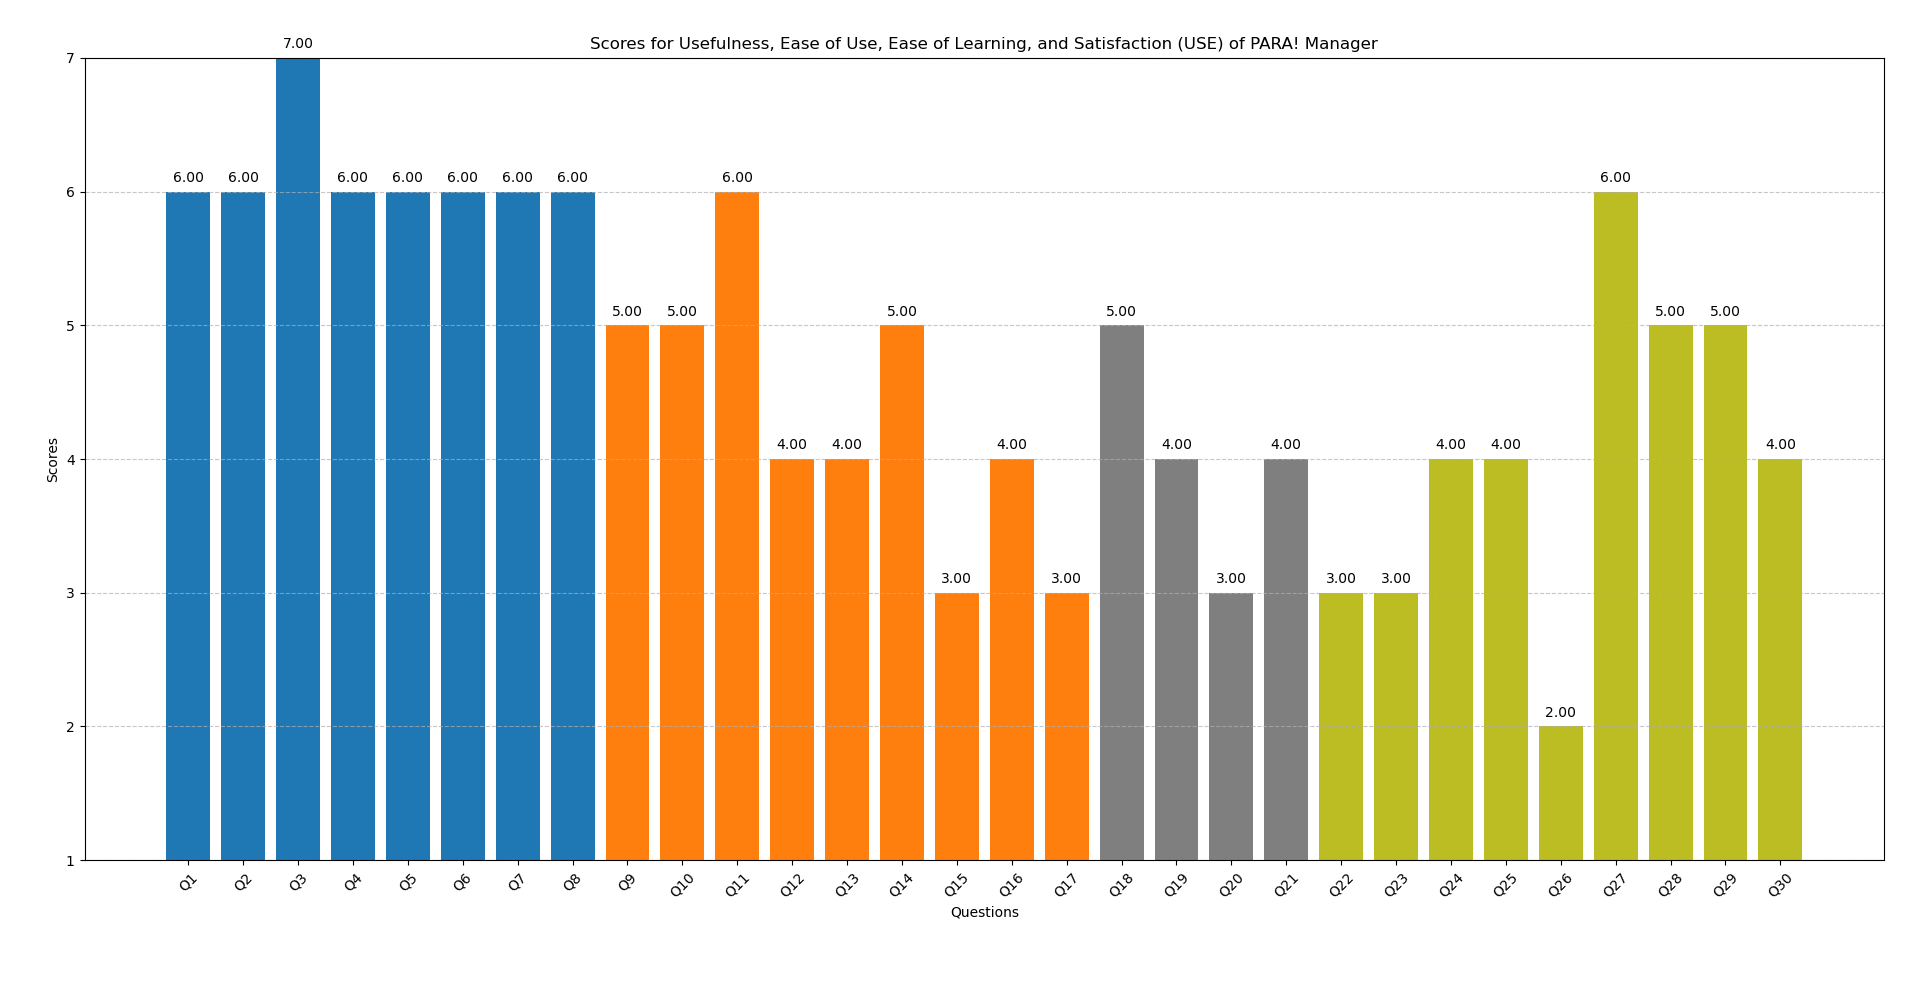
\includegraphics[scale=0.18]{./figures/manager means.png}
    \caption{Mean Scores for Usefulness, Ease of Use, Ease of Learning, and Satisfaction (USE) of PARA! Manager}
\end{figure}
\subsubsection{Usefulness}
Figure 13 shows the scores for each of the questions on the usefulness scale.
”It helps me be more effective” got 6.00, ”It helps me be more productive” got 6.00, ”It is useful” got 7.00, ”It gives me more control over the activities in my life” got 6.00, ”It makes the things I want to accomplish easier to get done” got 6.00, ”It saves me time when I use it” got 6.00, ”It meets my needs” got 6.00, ”It does everything I would expect it to do” got 6.00.
All the questions under usefulness got a score between 6 (agree) and 7 (strongly agree) with 6 being more dominant.
\subsubsection{Ease of Use}
Figure 13 shows the scores for each of the questions on the ease of use scale. ”It is easy to use” got 5.00, ”It is simple to use” got 5.00, ”It is user friendly” got 6.00, ”It is flexible” got 7.00, ”It requires the fewest steps possible to accomplish what I want to do with it” got 4.00, ”Using it is effortless” got 4.00, ”I can use it without written instructions” got 3.00, ”I don’t notice any inconsistencies as I use it” got 5.00, ”Both occasional and regular users would like it” got 2.00, ”I can recover from mistakes quickly and easily” got 4.00, ”I can use it successfully every time” got 4.00.
The questions under ease of use got scores between 3 (disagree) and 7 (strongly agree).
\subsubsection{Ease of Learning}
Figure 13 shows the scores for each of the questions on the ease of learning scale. ”I learned to use it quickly” got 3.00, ”I easily remember how to use it” got 4.00, ”It is easy to learn to use it” got 3.00, ”I quickly became skillful with it” got 3.00.
All of the questions under ease of learning got a score between 3 (somewhat disagree) and 4 (neutral).
\subsubsection{Satisfaction}
Figure 13 shows the scores for each of the questions on the usefulness scale. ”I am satisfied with it” got 5.00, ”I would recommend it to a friend” got 6.00, ”It is fun to use” got 2.00, ”It works the way I want it to work” got 4.00, ”It is wonderful” got 4.00, ”I feel I need to have it” got 6.00, ”It is pleasant to use” got 4.00.
\begin{figure}[h]
    \centering
        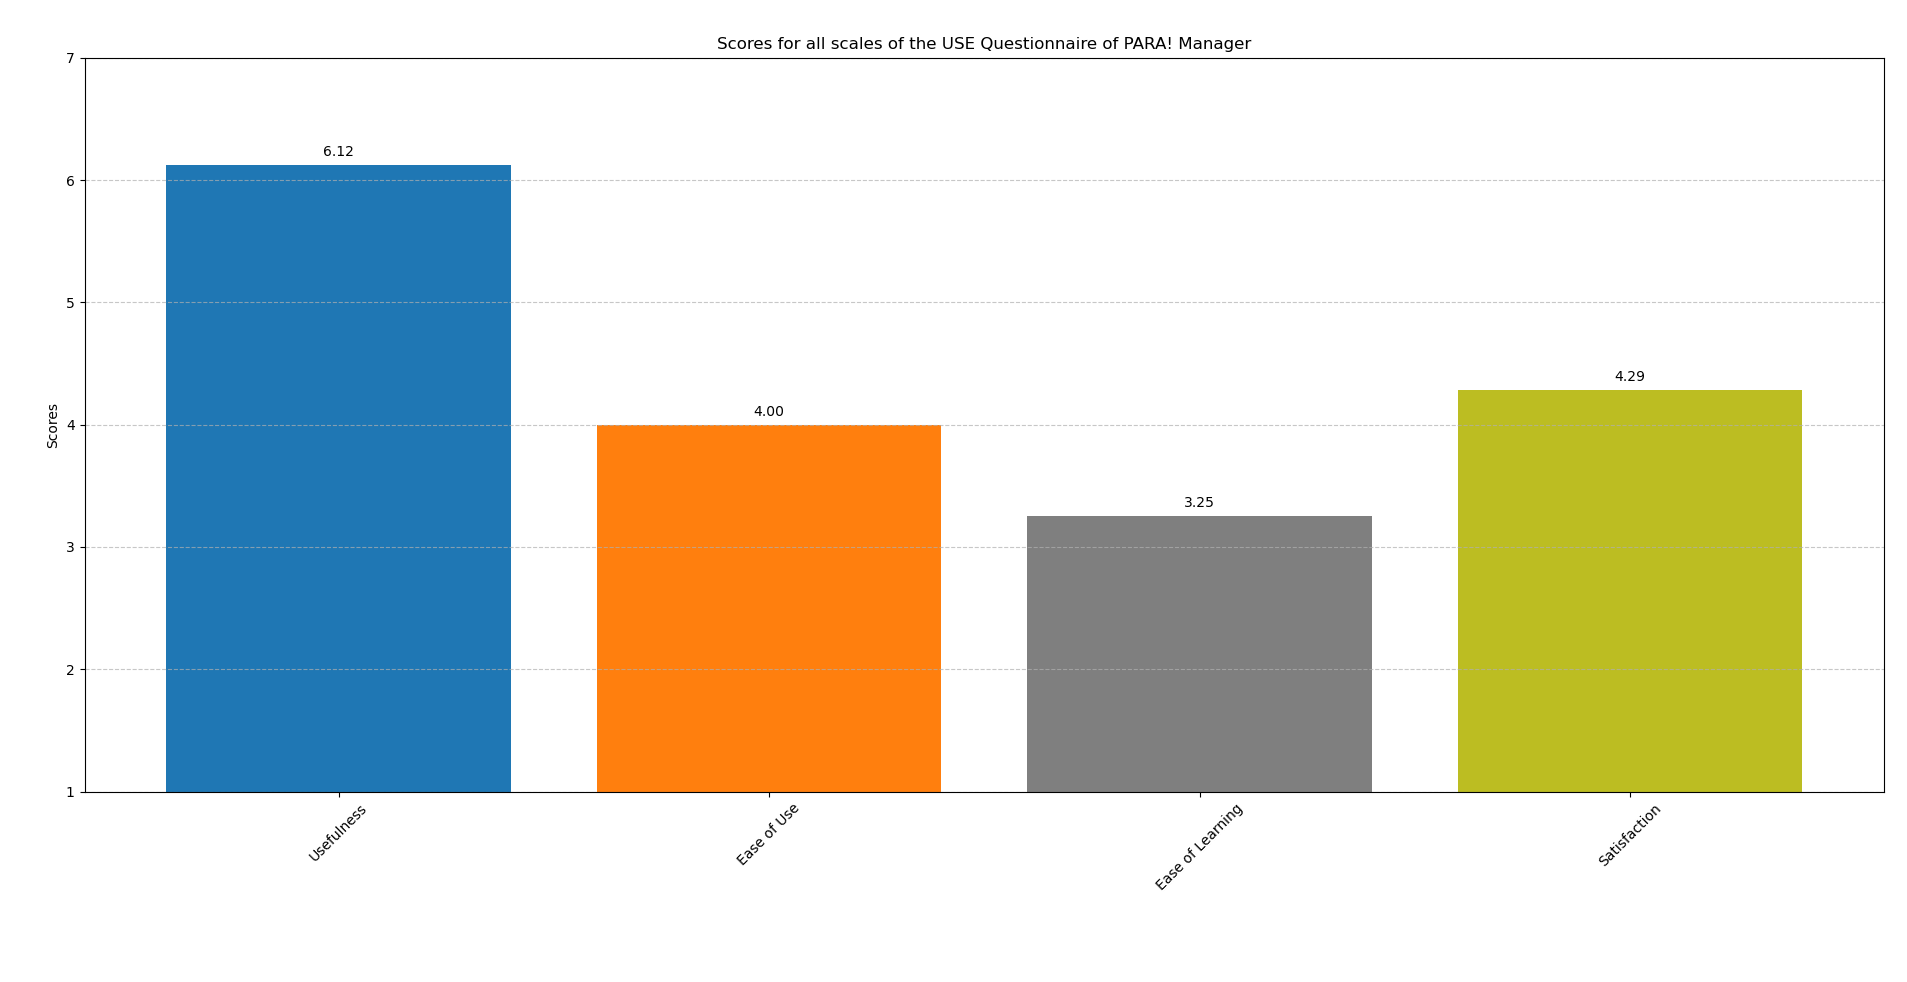
\includegraphics[scale=0.18]{./figures/manager means total.png}
    \caption{Mean Scores for Usefulness, Ease of Use, Ease of Learning, and Satisfaction (USE) of PARA! Manager}
\end{figure}
All of the questions under usefulness got a score between 6 (agree) and 7 (strongly agree).
\subsubsection{Interpretation}
Figure 14 shows the scores for all scales of the USE Questionnaire.
Usefulness got 6.12, Ease of Use got 4.00, Ease of Learning got 3.25, Satisfaction got 4.29.
The Usefulness scale got a score between 6 (agree) and 7 (strongly agree), meaning the participant overall agree to the usefulness of management application.
The Ease of Use scale got a score of 4 (neutral), indicating that the participant are neutral in agreeing or disagreeing with the ease of use of the management application.
The Ease of Learning scale got a score between 3 (somewhat disagree) and 4 (neutral), suggesting that the participant somewhat disagrees or is not sure about the ease of learning  of the management application.
The Satisfaction scale got scores between 4 (neutral) and 5 (somewhat agree), indicating that the participant are neutral to somewhat agreeing with the ease of use and satisfaction of the management application.
\subsubsection{Key Qualitative Assessment Points}
\begin{description}
    \item 1) The management app provides a better experience than manual data entry from Excel sheets.
    \item 2) It helps visualize the work slightly better compared to traditional methods.
    \item 3) However, the app has a steep learning curve.
\end{description}

\subsection{Client-facing application}
\begin{figure}[h]
    \centering
        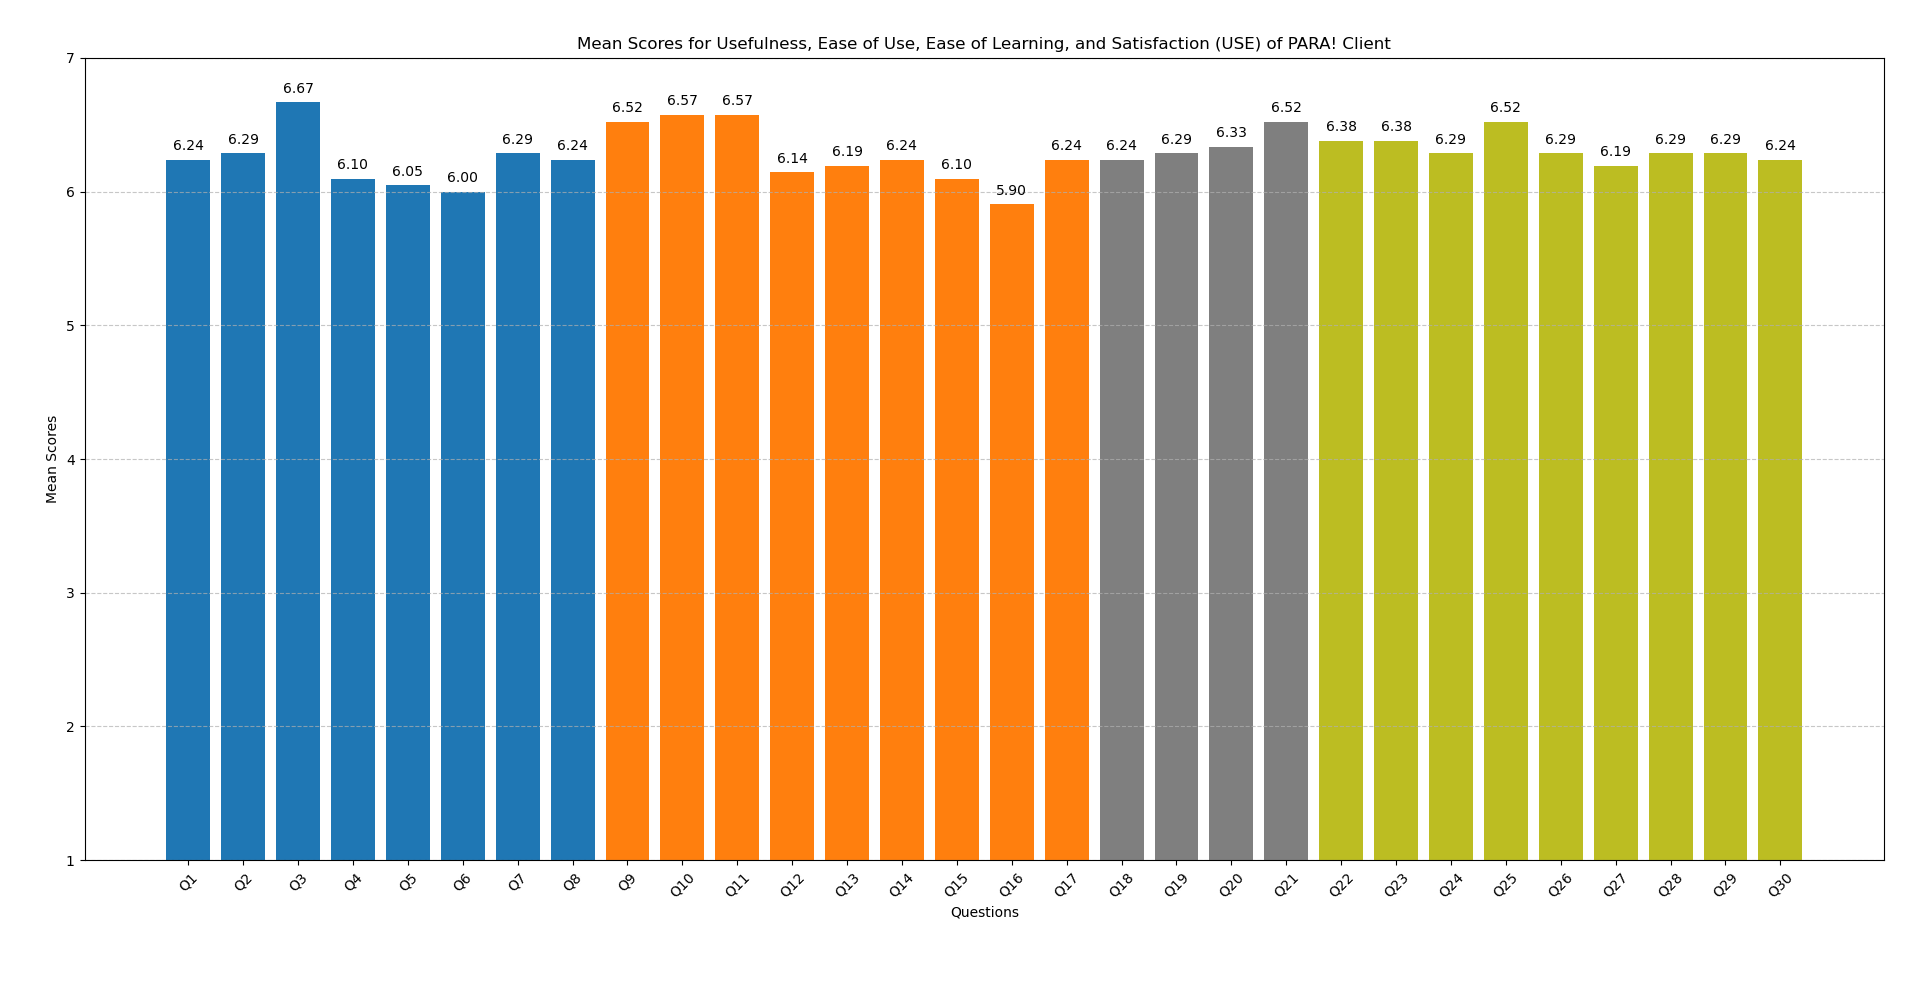
\includegraphics[scale=0.18]{./figures/client means.png}
    \caption{Mean Scores for Usefulness, Ease of Use, Ease of Learning, and Satisfaction (USE) of PARA! Client}
\end{figure}

\subsubsection{Usefulness}
Figure 15 on the next page shows the mean scores for each of the questions on the usefulness scale.
”It helps me be more effective” got 6.24, ”It helps me be more productive” got 6.29, ”It is useful” got 6.67, ”It gives me more control over the activities in my life” got 6.10, ”It makes the things I want to accomplish easier to get done” got 6.05, ”It saves me time when I use it” got 6.00, ”It meets my needs” got 6.29, ”It does everything I would expect it to do” got 6.24.
All the questions under usefulness got a mean score between 6 (agree) and 7 (strongly agree).
\subsubsection{Ease of Use}
Figure 15 shows the mean scores for each of the questions on the ease of use scale. ”It is easy to use” got 6.52, ”It is simple to use” got 6.57, ”It is user friendly” got 6.57, ”It is flexible” got 6.14, ”It requires the fewest steps possible to accomplish what I want to do with it” got 6.19, ”Using it is effortless” got 6.24, ”I can use it without written instructions” got 6.10, ”I don’t notice any inconsistencies as I use it” got 5.90, ”Both occasional and regular users would like it” got 6.24, ”I can recover from mistakes quickly and easily” got 6.24, ”I can use it successfully every time” got 6.29.
All the questions under ease of use got a mean score between 6 (agree) and 7 (strongly agree) except for the question "I don't notice any inconsistencies as I use it" which got 5.90 but is still within the agree range.
\subsubsection{Ease of Learning}
Figure 15 shows the mean scores for each of the questions on the ease of learning scale. ”I learned to use it quickly” got 6.33, ”I easily remember how to use it” got 6.52, ”It is easy to learn to use it” got 6.38, ”I quickly became skillful with it” got 6.38.
All of the questions under ease of learning got a mean score between 6 (agree) and 7 (strongly agree).
\subsubsection{Satisfaction}
Figure 15 shows the mean scores for each of the questions on the usefulness scale. ”I am satisfied with it” got 6.29, ”I would recommend it to a friend” got 6.52, ”It is fun to use” got 6.28, ”It works the way I want it to work” got 6.19, ”It is wonderful” got 6.29, ”I feel I need to have it” got 6.29, ”It is pleasant to use” got 6.24.
All of the questions under usefulness got a mean score between 6 (agree) and 7 (strongly agree).
\begin{figure}[h]
    \centering
        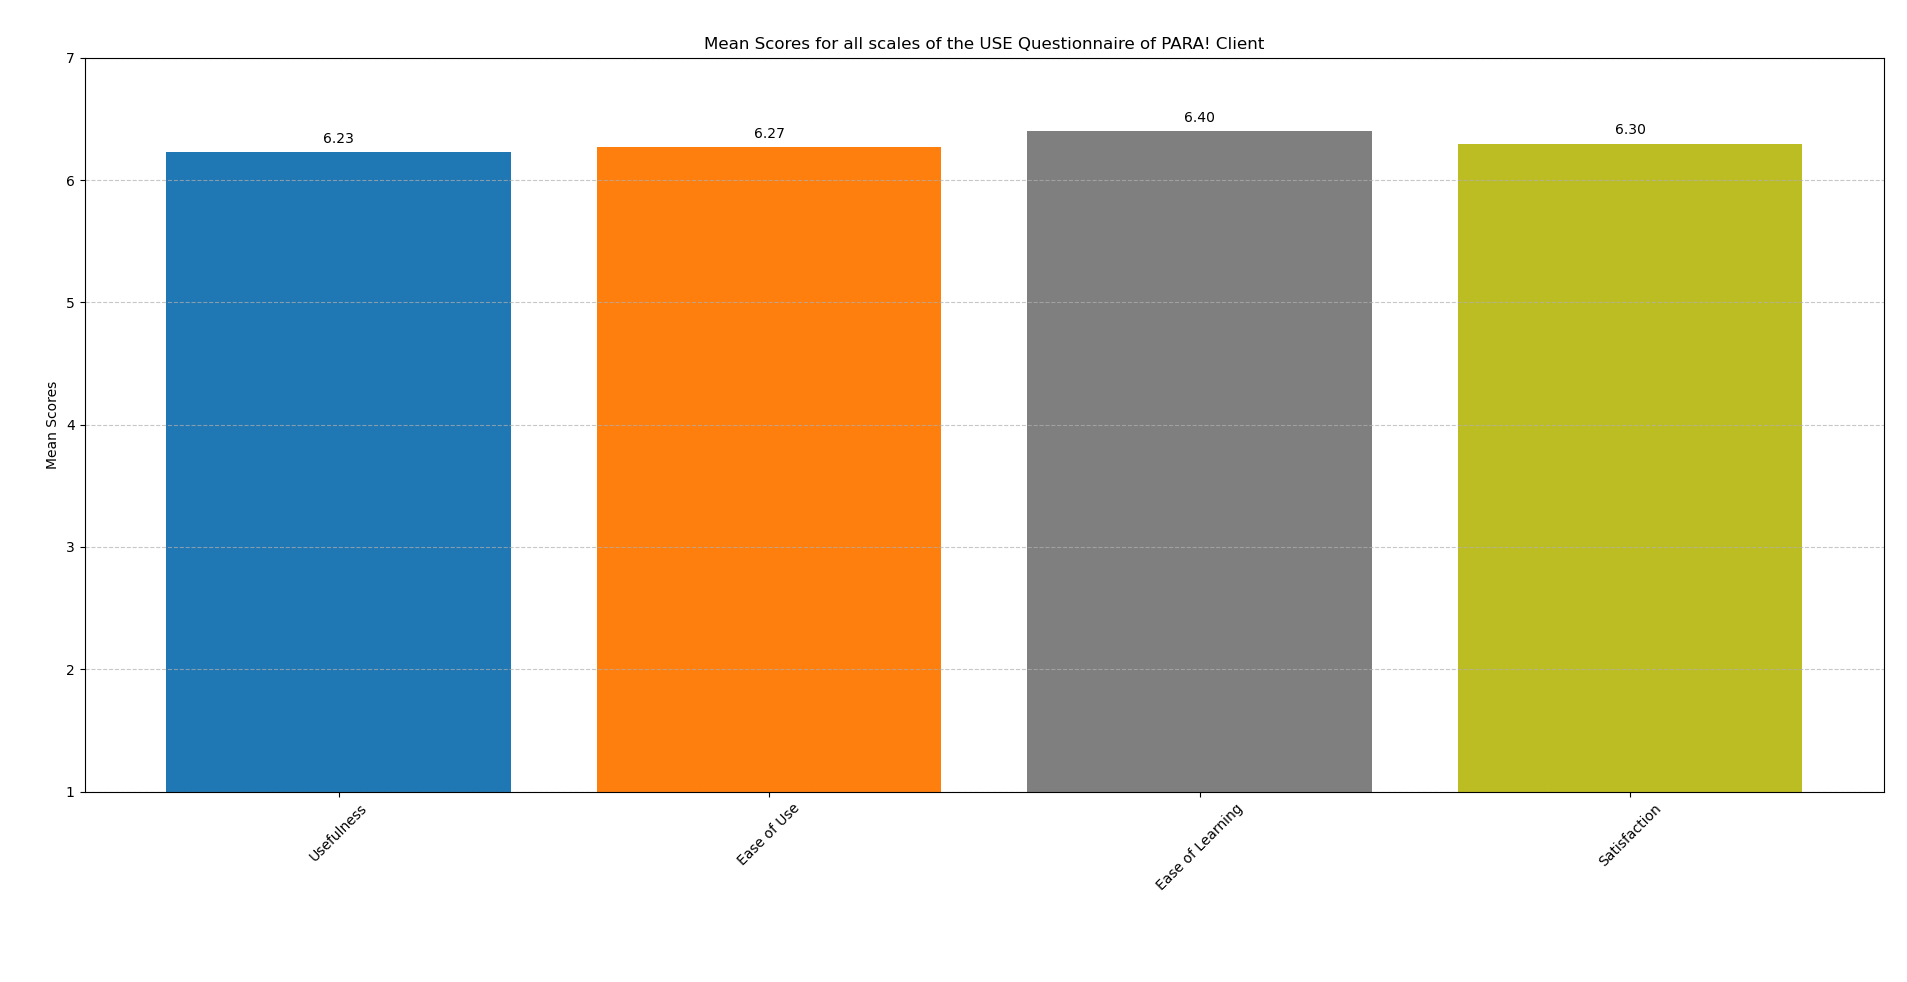
\includegraphics[scale=0.18]{./figures/client means total.png}
    \caption{Mean Scores for Usefulness, Ease of Use, Ease of Learning, and Satisfaction (USE) of PARA! Client}
\end{figure}
\subsubsection{Interpretation}
Figure 16 shows the mean scores for all scales of the USE Questionnaire. Usefulness got 6.23, Ease of Use got 6.27, Ease of Learning got 6.40, Satisfaction got 6.30.
All of the scales got a mean score between 6 (agree) and 7 (strongly agree), meaning respondents overall agree-strongly agree to the usefulness, ease of use, ease of learning, and satisfaction of PARA!.
\subsubsection{Key Qualitative Assessment Points}
\begin{description}
    \item 1) Users found the app useful for commuters, with potential to help traffic enforcers and other commuters.
    \item 2) Suggestions for improvement included using brighter colors for route lines, adjusting font sizes, specifying areas where the app can be used, including public transport options, and allowing users to save previous itineraries.
    \item 3) Some UI elements like the upper and lower parts of the landing page were seen as too invasive on the map view when starting a destination.
    \item 4) The app was seen to have potential to assist both locals and tourists if expanded to cover the whole country.
\end{description}
% CONCLUSION AND FUTURE WORK
\section{Conclusion and Future Work}
PARA! was successful in addressing the objectives and alleviating the challenges faced by commuters in the Philippines. The client-facing application, with its high scores across various metrics, indicates strong potential for real-world application. However, improvements are needed in the management application, particularly in terms of ease of use and ease of learning.

Future work should focus on refining the management application interface to make it more intuitive and user-friendly. Additional testing on a broader demographic could also provide more insights into user experience improvements. Furthermore, expanding the scope of the application to support more regions and transportation modes could increase its utility and impact.

Additionally, the expansion of this system calls for contributions to OpenTripPlanner and other mapping technologies that have OpenStreetMap at its core. PARA! will be released as an open source project to inspire budding developers and serve as basis for mapping and transit applications in the context of the Philippines.


\newpage

% APPENDICES
\appendices

\section{}
\begin{figure}[!h]
    \centering
        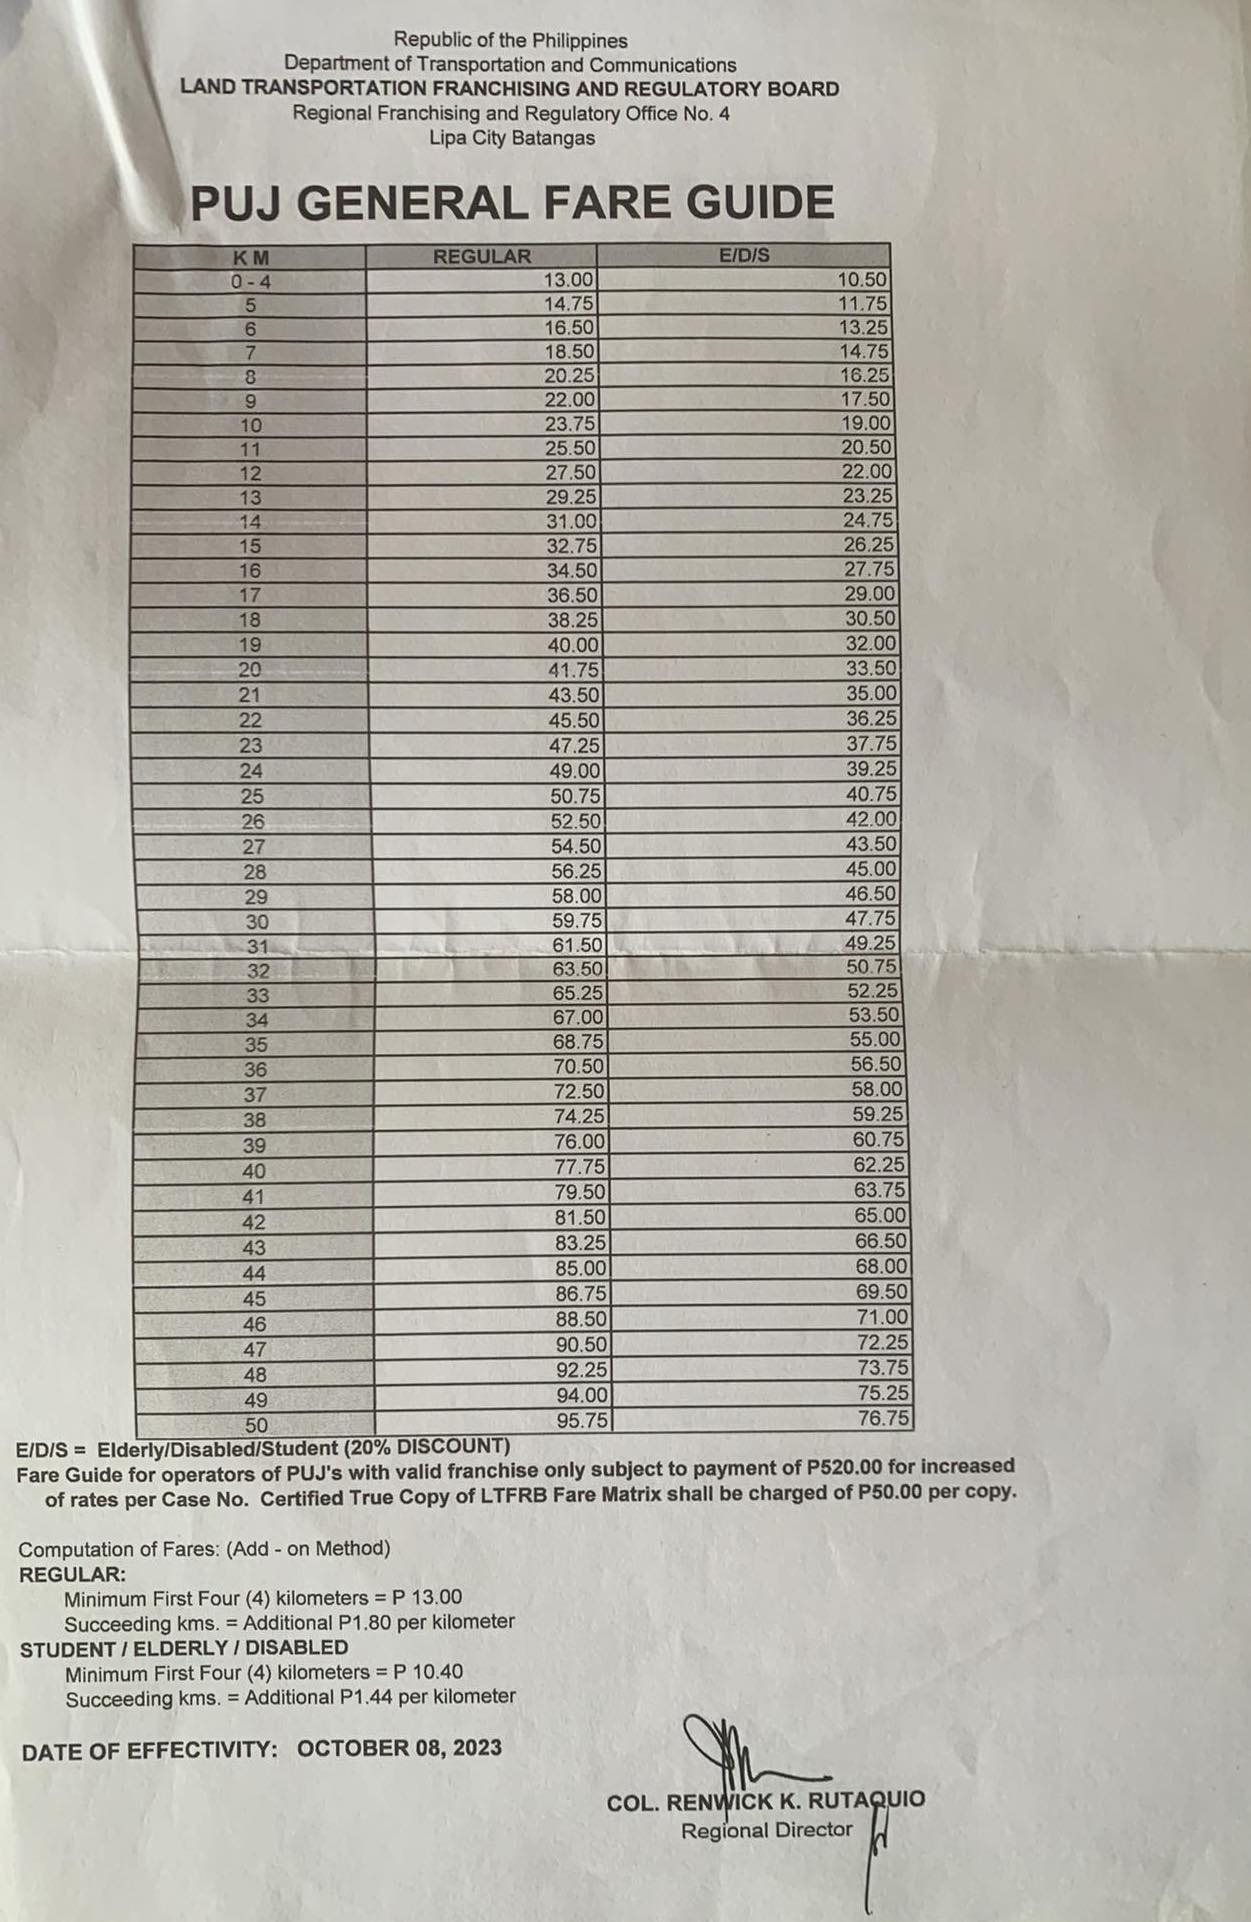
\includegraphics[scale=0.14]{./figures/ltfrb/puj.jpeg}
    \caption{PUJ General fare guide}
\end{figure}

\section{}
\begin{figure}[!h]
    \centering
        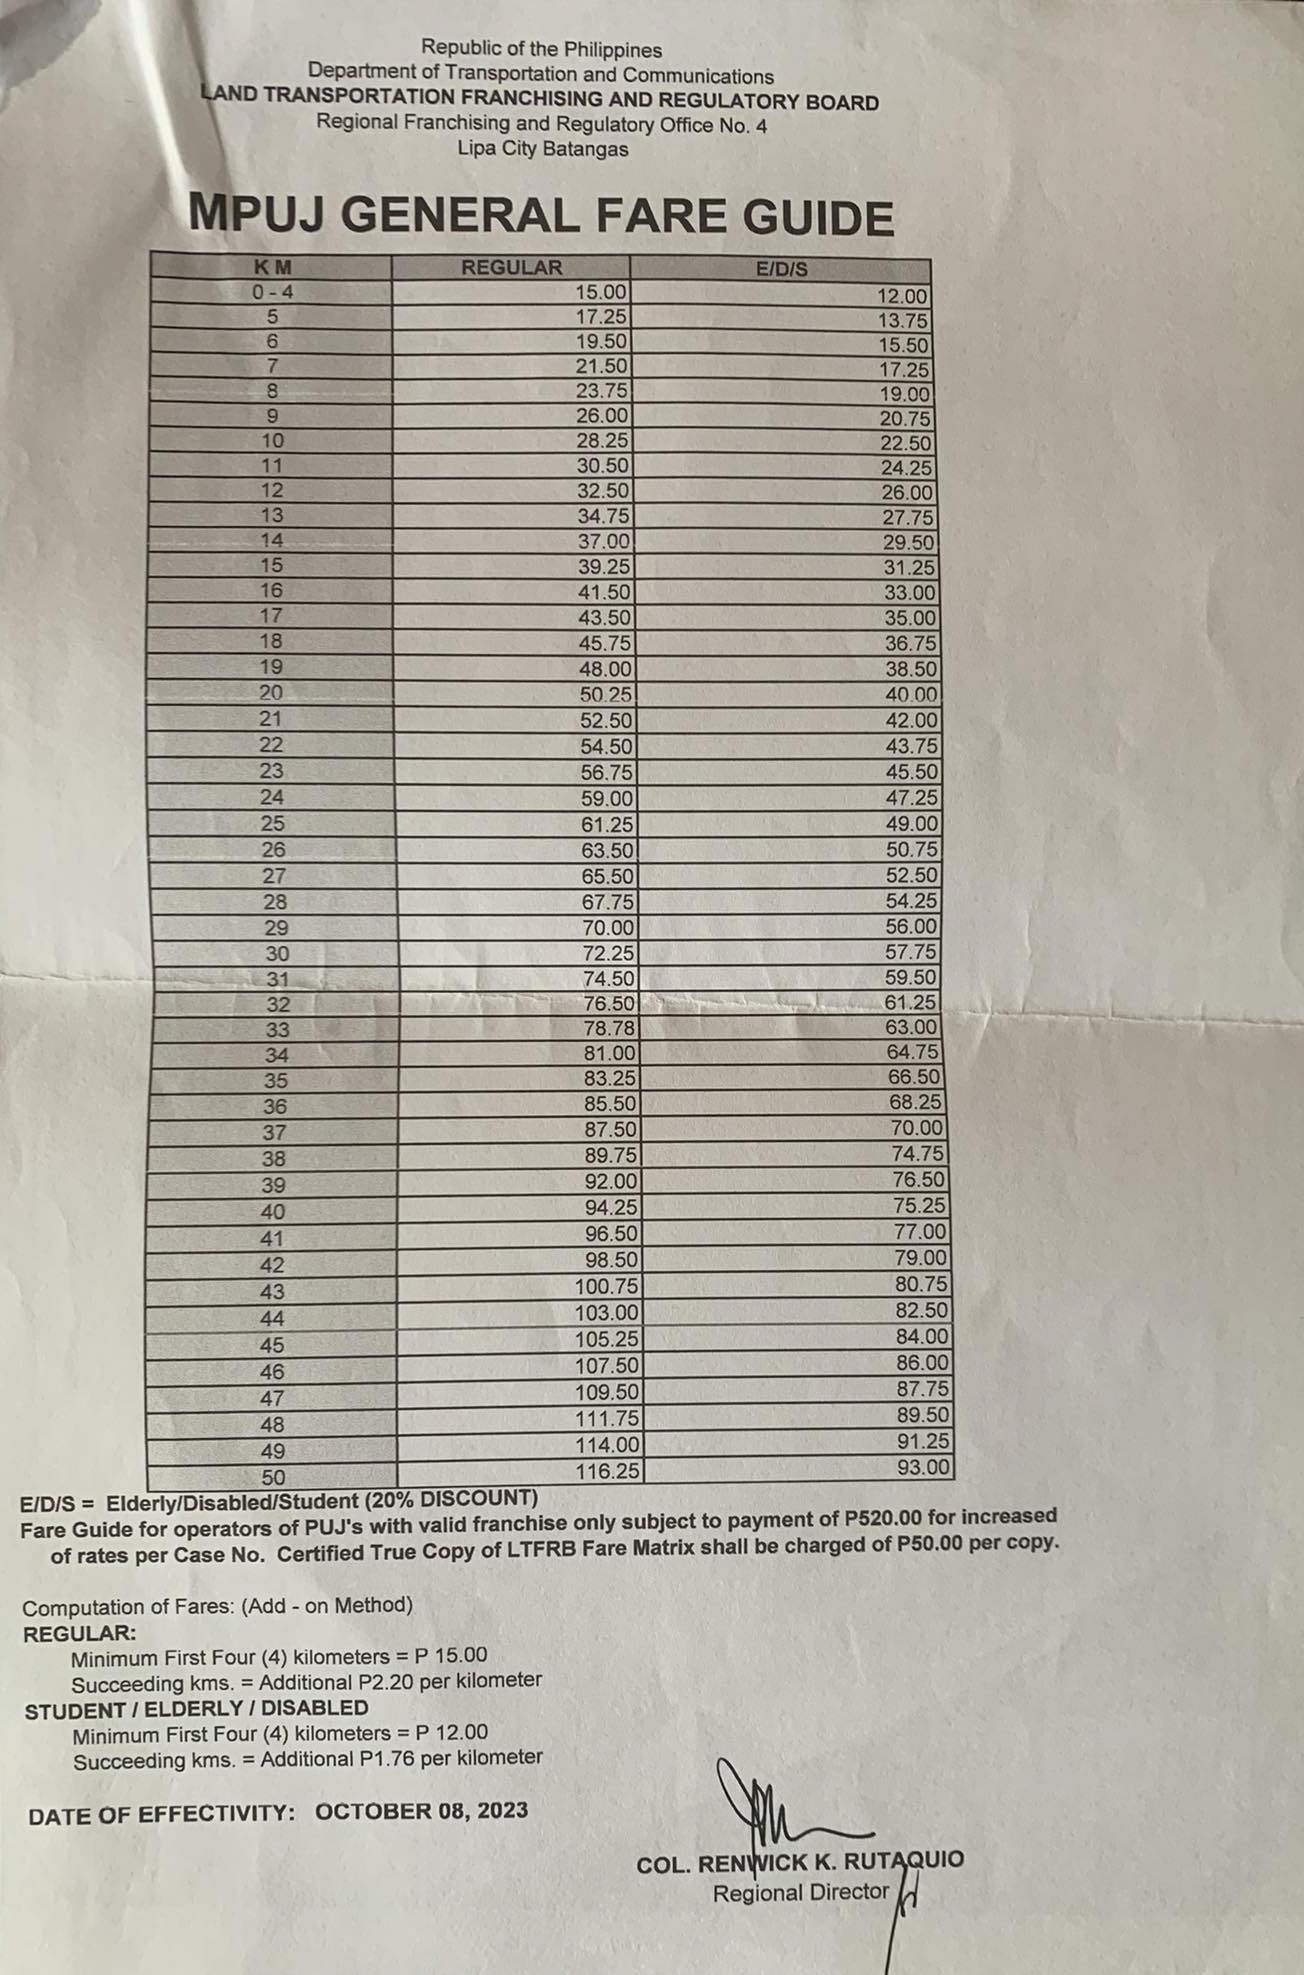
\includegraphics[scale=0.14]{./figures/ltfrb/mpuj.jpeg}
    \caption{MPUJ General fare guide}
\end{figure}

\newpage

\section{}
\begin{figure}[!h]
    \centering
        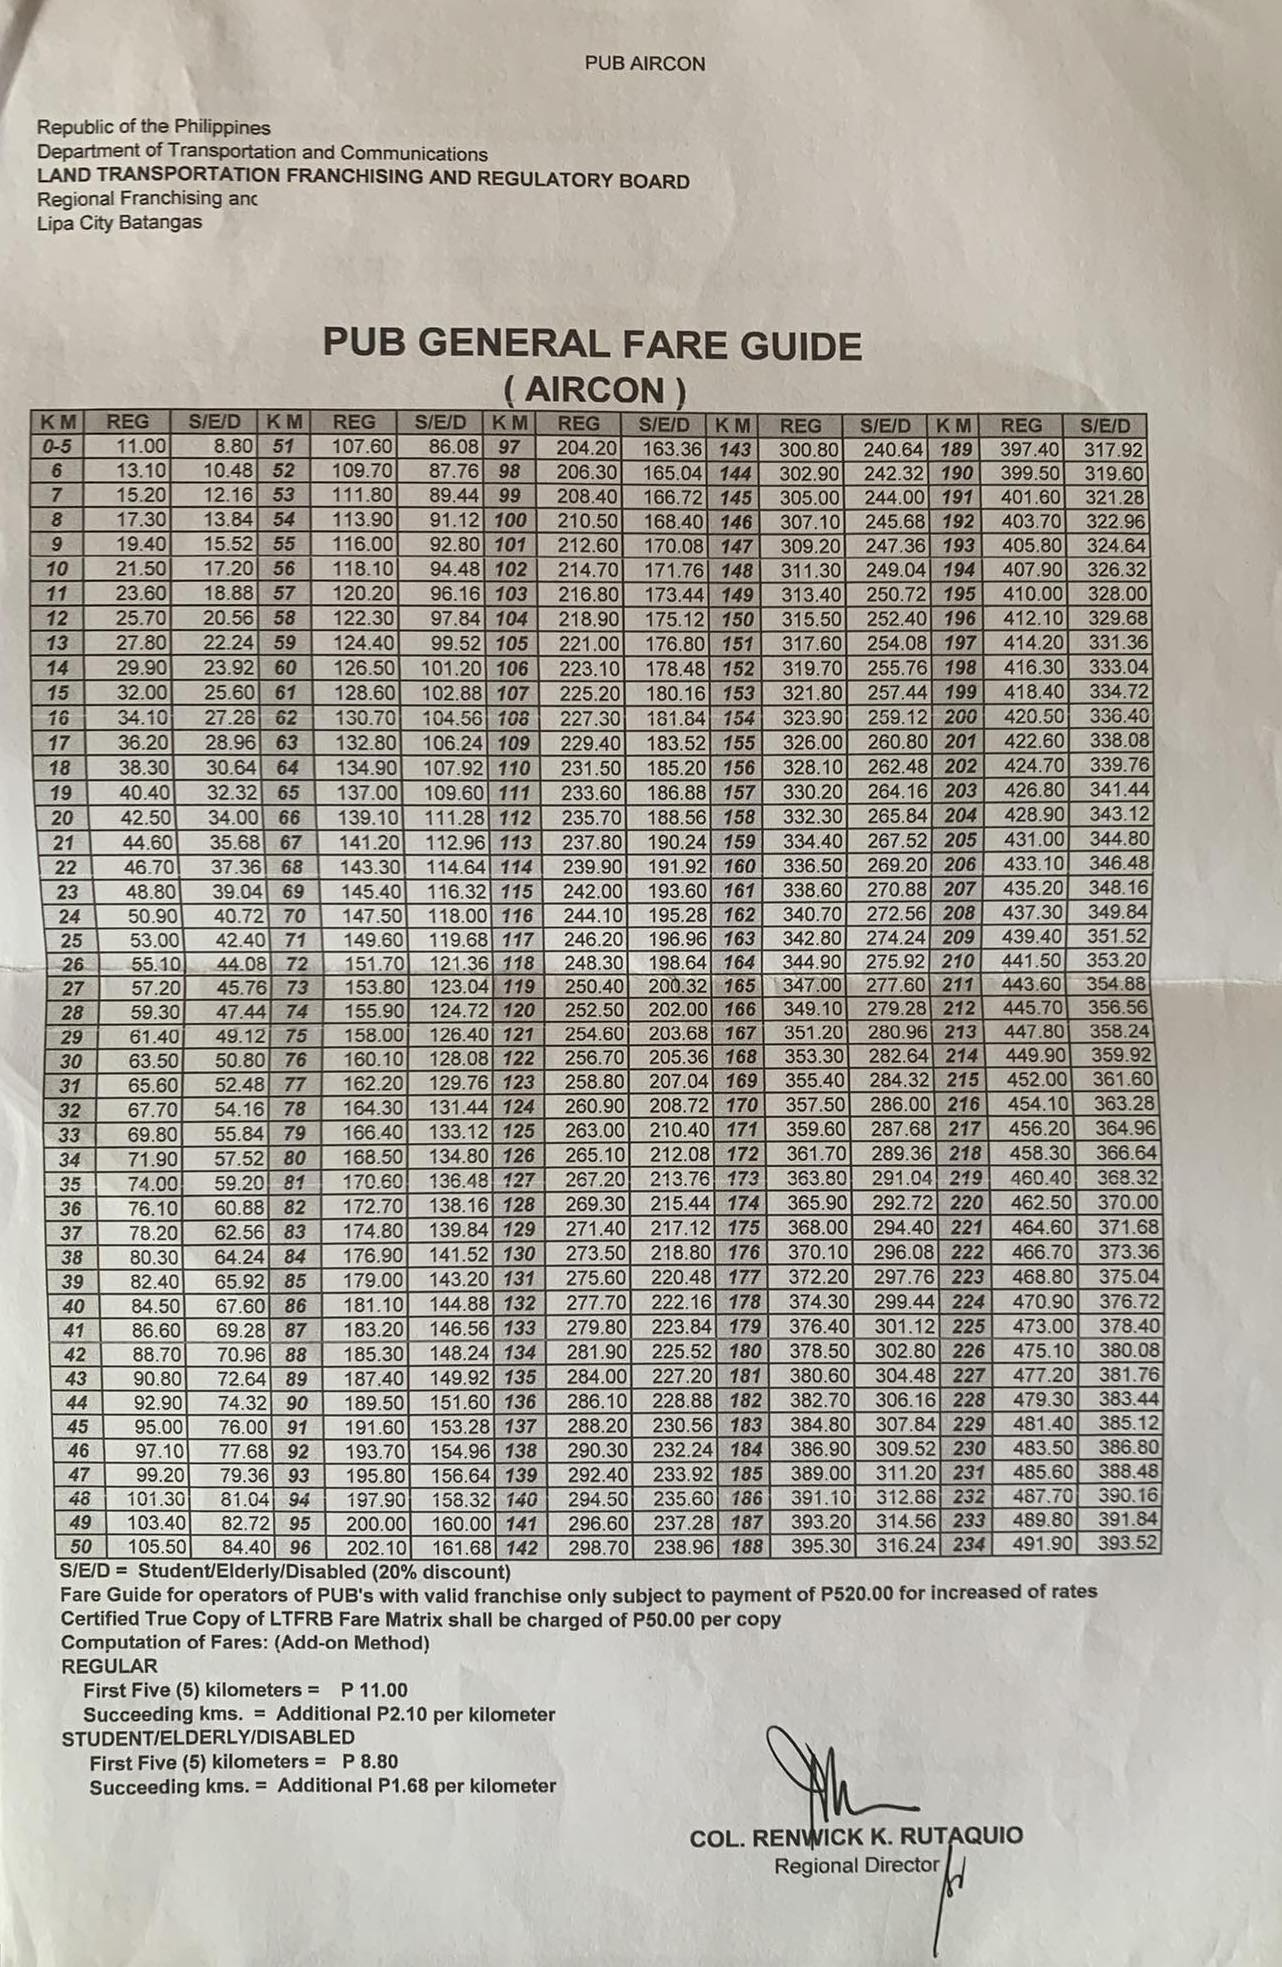
\includegraphics[scale=0.14]{./figures/ltfrb/pub.jpeg}
    \caption{PUB General fare guide}
\end{figure}

\section{}
\begin{figure}[!h]
    \centering
        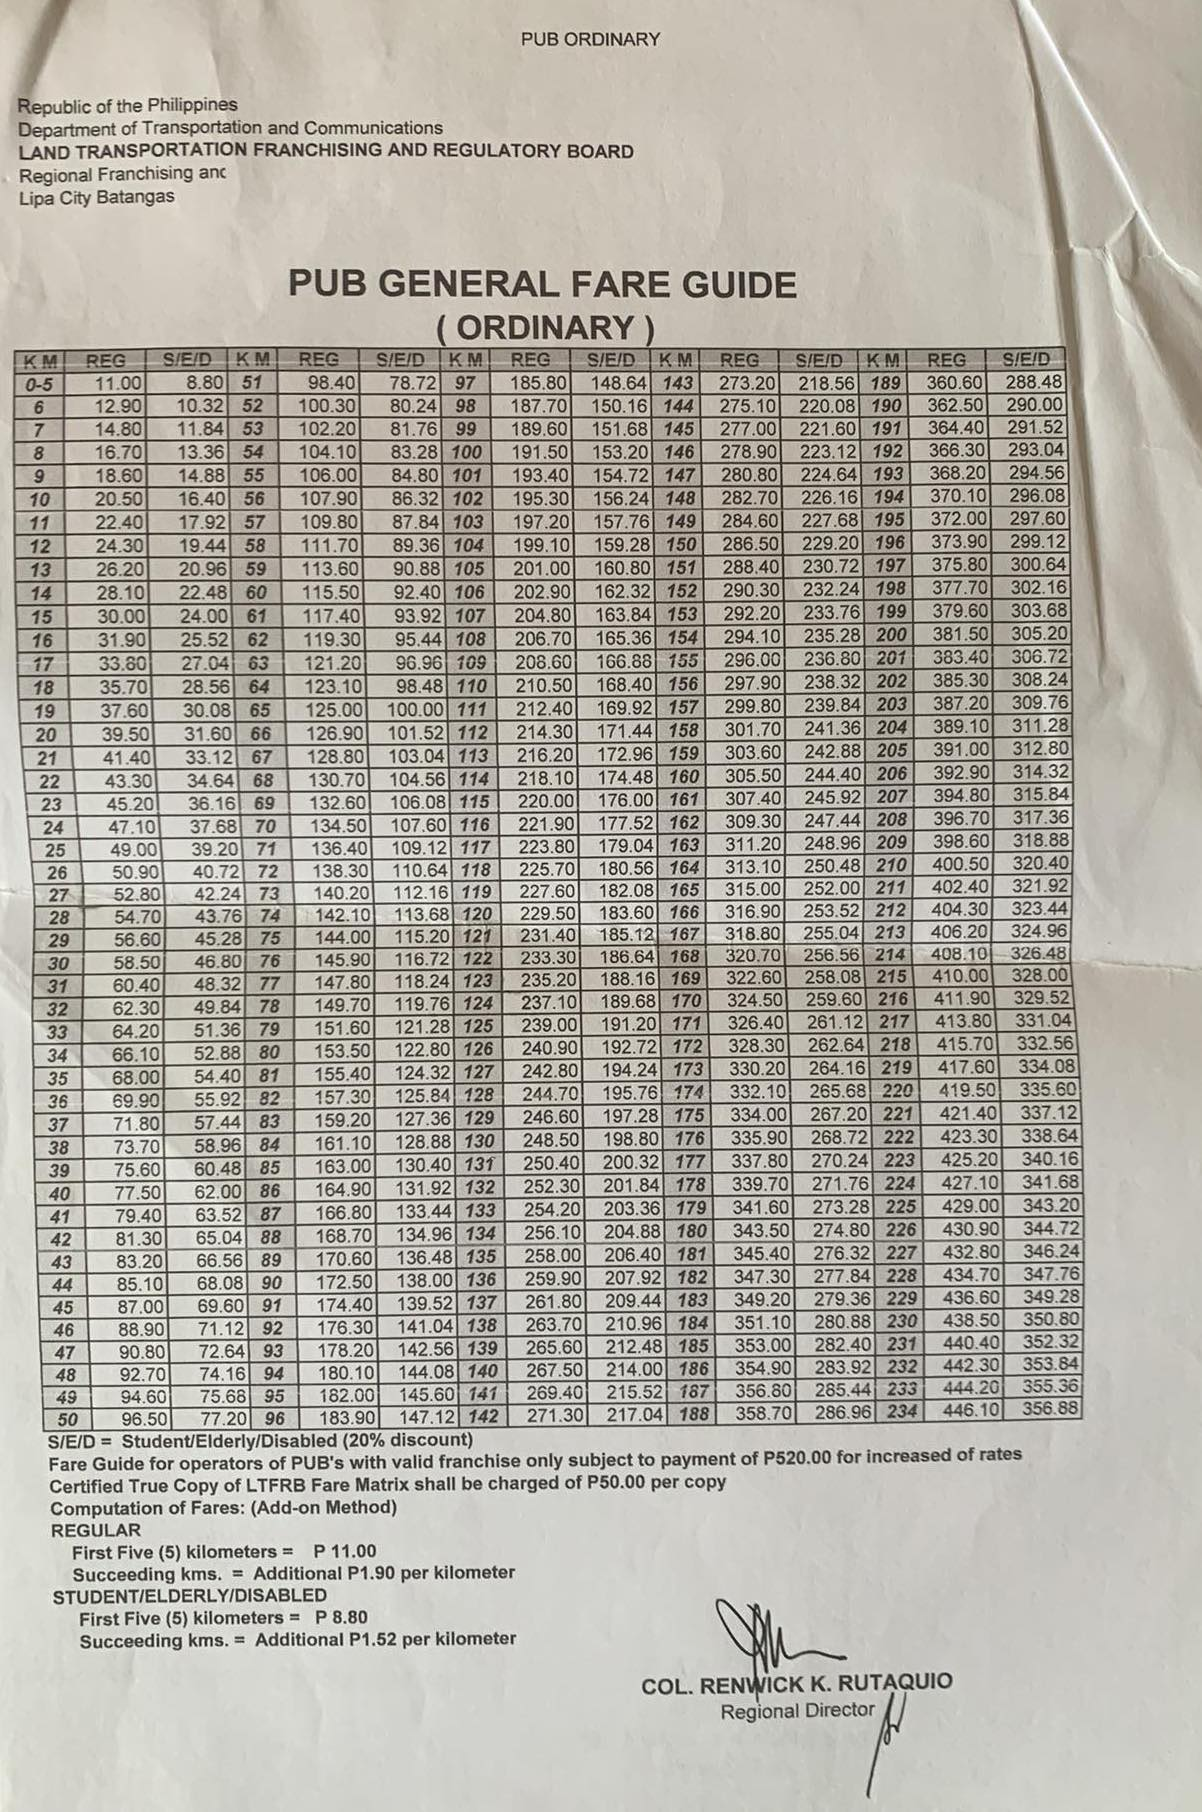
\includegraphics[scale=0.14]{./figures/ltfrb/pub ordinary.jpeg}
    \caption{PUB (ordinary) General fare guide}
\end{figure}



% ACKNOWLEDGMENT
\section*{Acknowledgment}
I would like to express my gratitude to my Special Problem adviser, Prof. Concepcion Khan, for her guidance. \hfill \\
Many thanks also to the open source communities of OpenStreetMap, Leaflet, OpenTripplanner, and Flutter Map, who answered my queries when no documentation could. \hfill \\
My utmost gratitude to my family who have been by my side from the beginning, providing me with the encouragement and support I needed to persevere. \hfill \\
To Angkol Junnie, one of the first comsci people who helped me have a smooth transition since my transfer from CAFS to CAS, I am thankful for everything that I learned from you. \hfill \\
To my loving girlfriend, Aliyah, you have my deepest love and appreciation for bringing out the best in me and inspiring me to develop this system. Without you, I could not have seen the things that mattered and because of you, I was able to really push myself to the limits more than I could have ever imagined.
% BIBLIOGRAPHY
\bibliographystyle{./IEEE/IEEEtran}
\bibliography{./atienza-sp-ieee}
% \nocite{*}

% BIOGRAPHY
\begin{biography}[{\includegraphics[scale=0.018]{./figures/sablay pic.jpg}}]{Jonas R. Atienza}
    is a Computer Science student from the University of the Philippines Los Baños. He is from Batangas City, Batangas. His research interests are cybersecurity, operating systems, geographic information systems (GIS), computer networks, and artificial intelligence (AI).
He highly believes in the power of Free Open Source Software (FOSS) and is very interested in contributing and developing technologies for the benefit of the people.
\end{biography}


\end{document}
 
